\documentclass[runningheads,11pt]{article}
\usepackage[margin=1in]{geometry}
\usepackage[utf8]{inputenc}
\usepackage[T1]{fontenc}
\usepackage{lmodern}
\usepackage{amsmath,amssymb,amsthm}
\usepackage{graphicx}
\usepackage{booktabs}
\usepackage{multirow}
\usepackage{caption}
\usepackage{subcaption}
\usepackage{siunitx}
\usepackage{microtype}
\usepackage[hidelinks]{hyperref}
\usepackage{cleveref}
\sisetup{group-separator={,}}
\graphicspath{{figures/}}
% Absorb minor line-end overflows from long \texttt{} tokens.
\emergencystretch=3em

\title{Iterative Re-estimation of Local Edge-Criticality Metrics
across Four Benchmark Networks}
\author{NetworkEntropy Research Project\\
\small Tokyo International University, 4-42-31 Higashi-Ikebukuro,
Toshima, Tokyo, Japan\\
\small \textbf{[Muhammad Kawser Ibn Kurshid Khan, vasily lubshevsky and ORCIDs to be completed]}}
\date{June 2026}

\begin{document}
\maketitle

\begin{abstract}
Identifying the edges whose removal fragments a complex network fastest is
central to attack-vulnerability analysis and to protecting critical
infrastructure: these links hold together otherwise separate parts of a network,
and finding them in advance can pre-empt cascading collapse. Many traditional indices
score edge criticality from a single, static view of the intact topology. But
every edge removal reshapes the graph, so a one-shot ranking drifts out of step
with the network it is dismantling. Deep Link Entropy and Improved Link Entropy
showed that recomputing a metric after \emph{each} removal works well, and we
apply the same step-by-step re-estimation to three local edge-criticality metrics
of increasing sophistication: Link Degree Centrality (LDC), Link-Local
Betweenness Centrality (LLBCe), and Link-Local Betweenness Mapping Entropy
(LLBMEe1). Using the relative-giant-component (RGC) curve and the area under it
(AUC; lower is better) as the decomposition-efficiency criterion, we benchmark
all three metrics, in both static and iterative form, on four real networks that
span a wide topological range: the Jazz musicians collaboration graph, the
Dolphins social network, a dense Baseball association graph, and a sparse urban
Transport network. Iterative re-estimation improves LLBCe and LLBMEe1 on
\emph{every} network, by mean AUC reductions of \SI{23.3}{\percent} and
\SI{32.7}{\percent} respectively and by up to \SI{43.7}{\percent}. For LDC the
benefit is conditional: iteration helps clearly on the sparse Transport and
Dolphins graphs but slightly degrades on the dense Jazz and Baseball graphs
(mean \SI{4.0}{\percent} loss), a negative result we report rather than hide.
Across all three metrics the gain from iteration grows as networks become
sparser and more bridge-dominated.
\end{abstract}

\noindent\textbf{Keywords:} Complex Networks, Edge Significance, Edge
Criticality, Link Degree Centrality, Link-Local Betweenness, Mapping Entropy,
Iterative Re-estimation, Network Robustness.

\section{Introduction}
\label{sec:intro}
Complex networks underpin much of modern infrastructure. Examples include
communication networks~\cite{onnela2007structure}, power-supply
networks~\cite{wang2017identification}, transport
systems~\cite{ghosh2011railway}, and biological systems such as protein-DNA
interaction graphs~\cite{newman2003structure}. As more sectors come to depend on
such networks, understanding how they withstand failure becomes necessary to
keep them running.

Network science draws on theories and methods from several disciplines. A
complex network can be examined through its topological structure or through the
criticality of its individual links, and both views help make networks harder to
fragment and pre-empt cascading failure. Researchers work in several directions: some predict
new connections to optimise a network~\cite{newman2003structure}; some rank
influential \emph{nodes} to assess resilience~\cite{albert2002statistical}; and
some study critical \emph{edges}, measuring the connectivity left after a link is
removed. Robustness research has mostly concentrated on node removal, and edge
removal is comparatively under-explored. This study addresses that gap by
removing edges rather than nodes.

Methods for evaluating edge criticality fall into two families.
\emph{Straightforward} algorithms analyse local topological features and assign
a criticality value to each edge independently. They include Edge
Betweenness~\cite{xia2008attack}, the Degree
Product~\cite{wang2008universal}, Bridgeness~\cite{cheng2010bridgeness},
Diffusion Importance, Topological Overlap~\cite{onnela2007structure}, $k$-path
centrality, and Link Entropy. Their strengths differ by network type: the Degree
Product does best on assortative networks, while Bridgeness does better on dense
graphs. \emph{Integral-optimisation} algorithms instead take a macro-level view;
the Evolutionary Approach~\cite{lubashevskiy2023evolutionary}, for example, uses
genetic principles to rank edges and can beat straightforward methods on ranking
quality, but at a much higher computational cost.

Two recent straightforward algorithms, Deep Link
Entropy~\cite{ozaydin2021deep} and Improved Link
Entropy~\cite{lubashevskiy2023improved}, both based on Link Entropy, improved
efficiency through \emph{iterative re-estimation}: recomputing the topological
feature after each edge removal so the ranking tracks the changing network. We
apply the same step-by-step re-evaluation to three local edge-criticality
metrics of increasing sophistication and compare their static and iterative
rankings:
\begin{itemize}
\item \textbf{Link Degree Centrality (LDC)}, a purely local degree-product
statistic;
\item \textbf{Link-Local Betweenness Centrality (LLBCe)}, edge betweenness
restricted to the first-order central domain of the edge; and
\item \textbf{Link-Local Betweenness Mapping Entropy (LLBMEe1)}, a metric
that couples an edge's local betweenness with the mapping entropy of its
neighbourhood.
\end{itemize}
We numerically decompose four well-known benchmark networks chosen to span a
wide topological range: the Jazz musicians network~\cite{gleiser2003jazz}, the
Dolphins social network~\cite{lusseau2003dolphins}, a dense Baseball association
graph, and a sparse, near-tree urban Transport network. For each we compare the
static and iterative variants under the relative-giant-component criterion. The
rest of the paper introduces the three metrics and the iterative principle
(\cref{sec:methods}), describes the data, decomposition procedure, and
per-network results (\cref{sec:setup}), discusses cross-cutting patterns and
limitations (\cref{sec:discussion}), and concludes (\cref{sec:conclusion}).

\section{Methods}
\label{sec:methods}
This section introduces the three edge-criticality metrics (LDC, LLBCe, and
LLBMEe1), then the iterative re-estimation principle applied to each, and finally
the decomposition-efficiency criterion used throughout.

\subsection{Link Degree Centrality (LDC)}
\label{sec:ldc}
Link Degree Centrality (LDC), also known as the degree product, scores an edge
by the product of the degrees of its two endpoints. It originates from work
describing cascading-failure-induced disasters in weighted
networks~\cite{wang2008universal}. For an edge $e=(u,v)$ in an undirected graph
$G=(V,E)$,
\begin{equation}
\mathrm{LDC}(e) \;=\; k_u \cdot k_v,
\label{eq:ldc}
\end{equation}
where $k_u$ and $k_v$ are the degrees of nodes $u$ and $v$, that is, the
number of edges incident on each endpoint. The idea is that an edge joining
two high-degree hubs carries a large share of the network's connectivity, so
removing it should fragment the giant component faster. LDC is a purely local,
$O(|E|)$ statistic and performs well on assortative networks, where high-degree
nodes tend to attach to one another~\cite{wang2008universal}. Edges are removed
in \emph{descending} LDC order.

\subsection{Link-Local Betweenness Centrality (LLBCe)}
\label{sec:llbce}
Classical edge betweenness scores an edge by counting the shortest paths between
all node pairs that pass through it~\cite{xia2008attack}; an edge on many
geodesics connects different parts of the network and is therefore critical.
Evaluating betweenness over \emph{all} node pairs is expensive. Link-Local
Betweenness Centrality (LLBCe) restricts the computation to the \emph{first-order
central domain} of the edge, which keeps it sensitive to bridging structure while
avoiding the global all-pairs cost~\cite{entropy2024llbme}. The construction has
three steps.

\paragraph{Step 1: central domain.}
For an edge $e=(u,v)$ define the first-order central domain
\begin{equation}
\Gamma(e) \;=\; \{u,v\}\,\cup\, N(u)\,\cup\, N(v),
\label{eq:gamma}
\end{equation}
the two endpoints together with all of their immediate neighbours. This local
set delimits the node pairs over which betweenness will be accumulated.

\paragraph{Step 2: restricted path counting.}
For each ordered pair $s,t\in\Gamma(e)$ let $\sigma_{st}$ be the number of
shortest paths between $s$ and $t$ in the \emph{full} graph and $\sigma_{st}(e)$
the number of those paths that pass through $e$. The ratio
$\sigma_{st}(e)/\sigma_{st}$ is the share of $s$-to-$t$ communication that relies
on $e$; geodesics are measured in the full graph, with no subgraph extraction.

\paragraph{Step 3: normalised aggregation.}
LLBCe is the average of these shares over the central domain,
\begin{equation}
\mathrm{LLBCe}(e) \;=\;
\frac{1}{|\Gamma(e)|\,(|\Gamma(e)|-1)}
\sum_{\substack{s,t\in\Gamma(e)\\ s\neq t}}
\frac{\sigma_{st}(e)}{\sigma_{st}}.
\label{eq:llbce}
\end{equation}
Normalising by $|\Gamma(e)|\,(|\Gamma(e)|-1)$, the number of ordered pairs in
the domain, makes scores comparable across edges whose neighbourhoods differ in
size. When the removal of $e$ disconnects $s$ and $t$ the corresponding term is
taken to be zero. Edges are removed in \emph{descending} LLBCe order.

\subsection{Link-Local Betweenness Mapping Entropy (LLBMEe1)}
\label{sec:llbme}
Link-Local Betweenness Mapping Entropy (LLBMEe1) combines the local betweenness
of an edge with the \emph{mapping entropy} of its neighbourhood, so it rewards
edges that are both locally central and sitting in a heterogeneous local
environment~\cite{entropy2024llbme}. Let $\mathrm{LLBCe}_{\mathrm{raw}}(e)$
denote the un-normalised Link-Local Betweenness of $e$, the inner sum of
\cref{eq:llbce} before the $|\Gamma(e)|(|\Gamma(e)|-1)$ division, and let
$N(e_1)$ be the set of edges sharing an endpoint with $e_1$. Then
\begin{equation}
\mathrm{LLBMEe1}(e_1) \;=\;
-\,\mathrm{LLBCe}_{\mathrm{raw}}(e_1)
\sum_{e_2\in N(e_1)} \log\!\bigl(\mathrm{LLBCe}_{\mathrm{raw}}(e_2)\bigr),
\label{eq:llbme}
\end{equation}
with the score set to $0$ when $\mathrm{LLBCe}_{\mathrm{raw}}(e_1)\le 0$ and the
logarithm floored at $\log(10^{-10})$ for numerical stability. The metric
combines two factors: the edge's own local betweenness, and the entropy-like
sum of the log-betweenness of its incident edges, which is large when the
neighbourhood is structurally diverse. The neighbour betweenness values are
usually below unity, so their logarithms are negative and \cref{eq:llbme} gives
\emph{negative} scores. The convention is therefore \emph{inverted criticality}:
the \emph{most negative} edge is the most critical, and edges are removed in
\emph{ascending} order (most negative first). The sign is not guaranteed
negative everywhere. If every neighbour's raw subset betweenness exceeds unity
the sum of logs is positive, and a few edges can flip sign. We monitor this, but
it does not change the ranking order materially on the networks studied here.

\subsection{Iterative Re-estimation}
\label{sec:iterative}
In the conventional, \emph{static} procedure a metric is evaluated once on the
intact graph, edges are ranked, and they are removed in that fixed order.
However, as the topology changes with each removal the criticality of the
surviving edges may change as well, so the initial ranking becomes progressively
stale. The \emph{iterative} variant addresses this by re-evaluating the metric
for every surviving edge after each removal and deleting the current
most-critical edge, repeating until the graph is fully dismantled. The procedure
is:
\begin{enumerate}
\item compute the metric for all edges of the current graph;
\item rank the edges and remove the single most-critical one;
\item record the size of the largest connected component and the fraction of
edges removed; and
\item repeat from step~1 on the reduced graph until no edges remain.
\end{enumerate}
This keeps the ranking aligned with the changing topology, the same principle
that sharpened Deep Link Entropy~\cite{ozaydin2021deep} and Improved Link
Entropy~\cite{lubashevskiy2023improved}, at the cost of repeated metric
evaluations. For LDC the recomputed quantity is the degree product; for LLBCe
and LLBMEe1 it is the local betweenness (and its mapping entropy) over each
edge's first-order central domain, recomputed on the current graph.

\subsection{Algorithm-Performance Measurement}
\label{sec:auc}
A network is decomposed by removing its edges in criticality order, and the
decomposition efficiency is read from the size of the largest connected
component as edges are removed. Let $\rho\in[0,1]$ be the fraction of edges
removed and $R_{gc}(\rho)$ the size of the largest connected component relative
to the original node count $N$. Initially $\rho=0$ and $R_{gc}=1$ (the graph is
connected); when the network is fully decomposed $\rho=1$ and $R_{gc}\to 0$.
The more critical the edges removed early, the more abruptly $R_{gc}$ falls as
$\rho$ grows, and the more efficient the ranking.

To summarise efficiency in a single number we use the area under the
$R_{gc}(\rho)$ curve,
\begin{equation}
\mathrm{AUC} \;=\; \int_0^1 R_{gc}(\rho)\,\mathrm{d}\rho,
\label{eq:auc}
\end{equation}
evaluated by the trapezoidal rule over the discrete removal sequence
$\{R_{gc}(i/|E|)\}_{i=0}^{|E|}$. This criterion emphasises the global features
of the decomposition rather than micro-level structure: a \emph{lower} AUC
indicates that critical edges were removed earlier and the network fragmented
faster, i.e.\ a more effective ranking. Throughout, $R_{gc}$ is normalised by
the node count and $\rho$ by the original edge count, so AUC values are directly
comparable across networks of different sizes.

\section{Data and Numerical Modelling}
\label{sec:setup}
To compare the static and iterative variants of LDC, LLBCe and LLBMEe1 we apply
the $R_{gc}(\rho)$ criterion to four real-world benchmark networks chosen to
span a wide topological range, from dense, highly clustered social graphs to a
sparse, near-tree spatial graph. All analysis is performed on the largest
connected component with self-loops removed. \Cref{tab:stats} reports their
structural statistics.

\begin{table}[t]
\centering
\caption{Structural statistics of the four benchmark networks (largest
connected component): nodes $N$, edges $E$, average degree $\langle k\rangle$,
maximum degree $k_{\max}$, degree heterogeneity
$H_k=\langle k^2\rangle/\langle k\rangle^2$, clustering coefficient $C$ and edge
density.}
\label{tab:stats}
\begin{tabular}{lccccccc}
\toprule
Network & $N$ & $E$ & $\langle k\rangle$ & $k_{\max}$ & $H_k$ & $C$ & density \\
\midrule
Jazz & 198 & 2742 & 27.70 & 100 & 1.395 & 0.618 & 0.1406 \\
Dolphins & 62 & 159 & 5.13 & 12 & 1.327 & 0.259 & 0.0841 \\
Baseball & 45 & 947 & 42.09 & 44 & 1.022 & 0.977 & 0.9566 \\
Transport & 369 & 430 & 2.33 & 7 & 1.190 & 0.029 & 0.0063 \\
\bottomrule
\end{tabular}
\end{table}

The four networks differ sharply in density and clustering. \textbf{Jazz} is a
dense, highly clustered musician-collaboration graph; \textbf{Dolphins} is a
small, sparse social network with a clear two-community structure;
\textbf{Baseball} is an almost-complete association graph ($C=0.977$, density
$0.957$); and \textbf{Transport} is a large, very sparse, nearly tree-like
spatial graph ($C=0.029$), where connectivity hinges on a few bridge edges.
\Cref{fig:circular} shows their circular layouts. In the
following subsections we decompose each network with the static and iterative
variants of the three metrics and describe the resulting $R_{gc}(\rho)$ curves;
the consolidated AUC values appear in \cref{tab:main} in \cref{sec:discussion}.

\begin{figure}[t]
\centering
\begin{subfigure}[t]{0.30\textwidth}
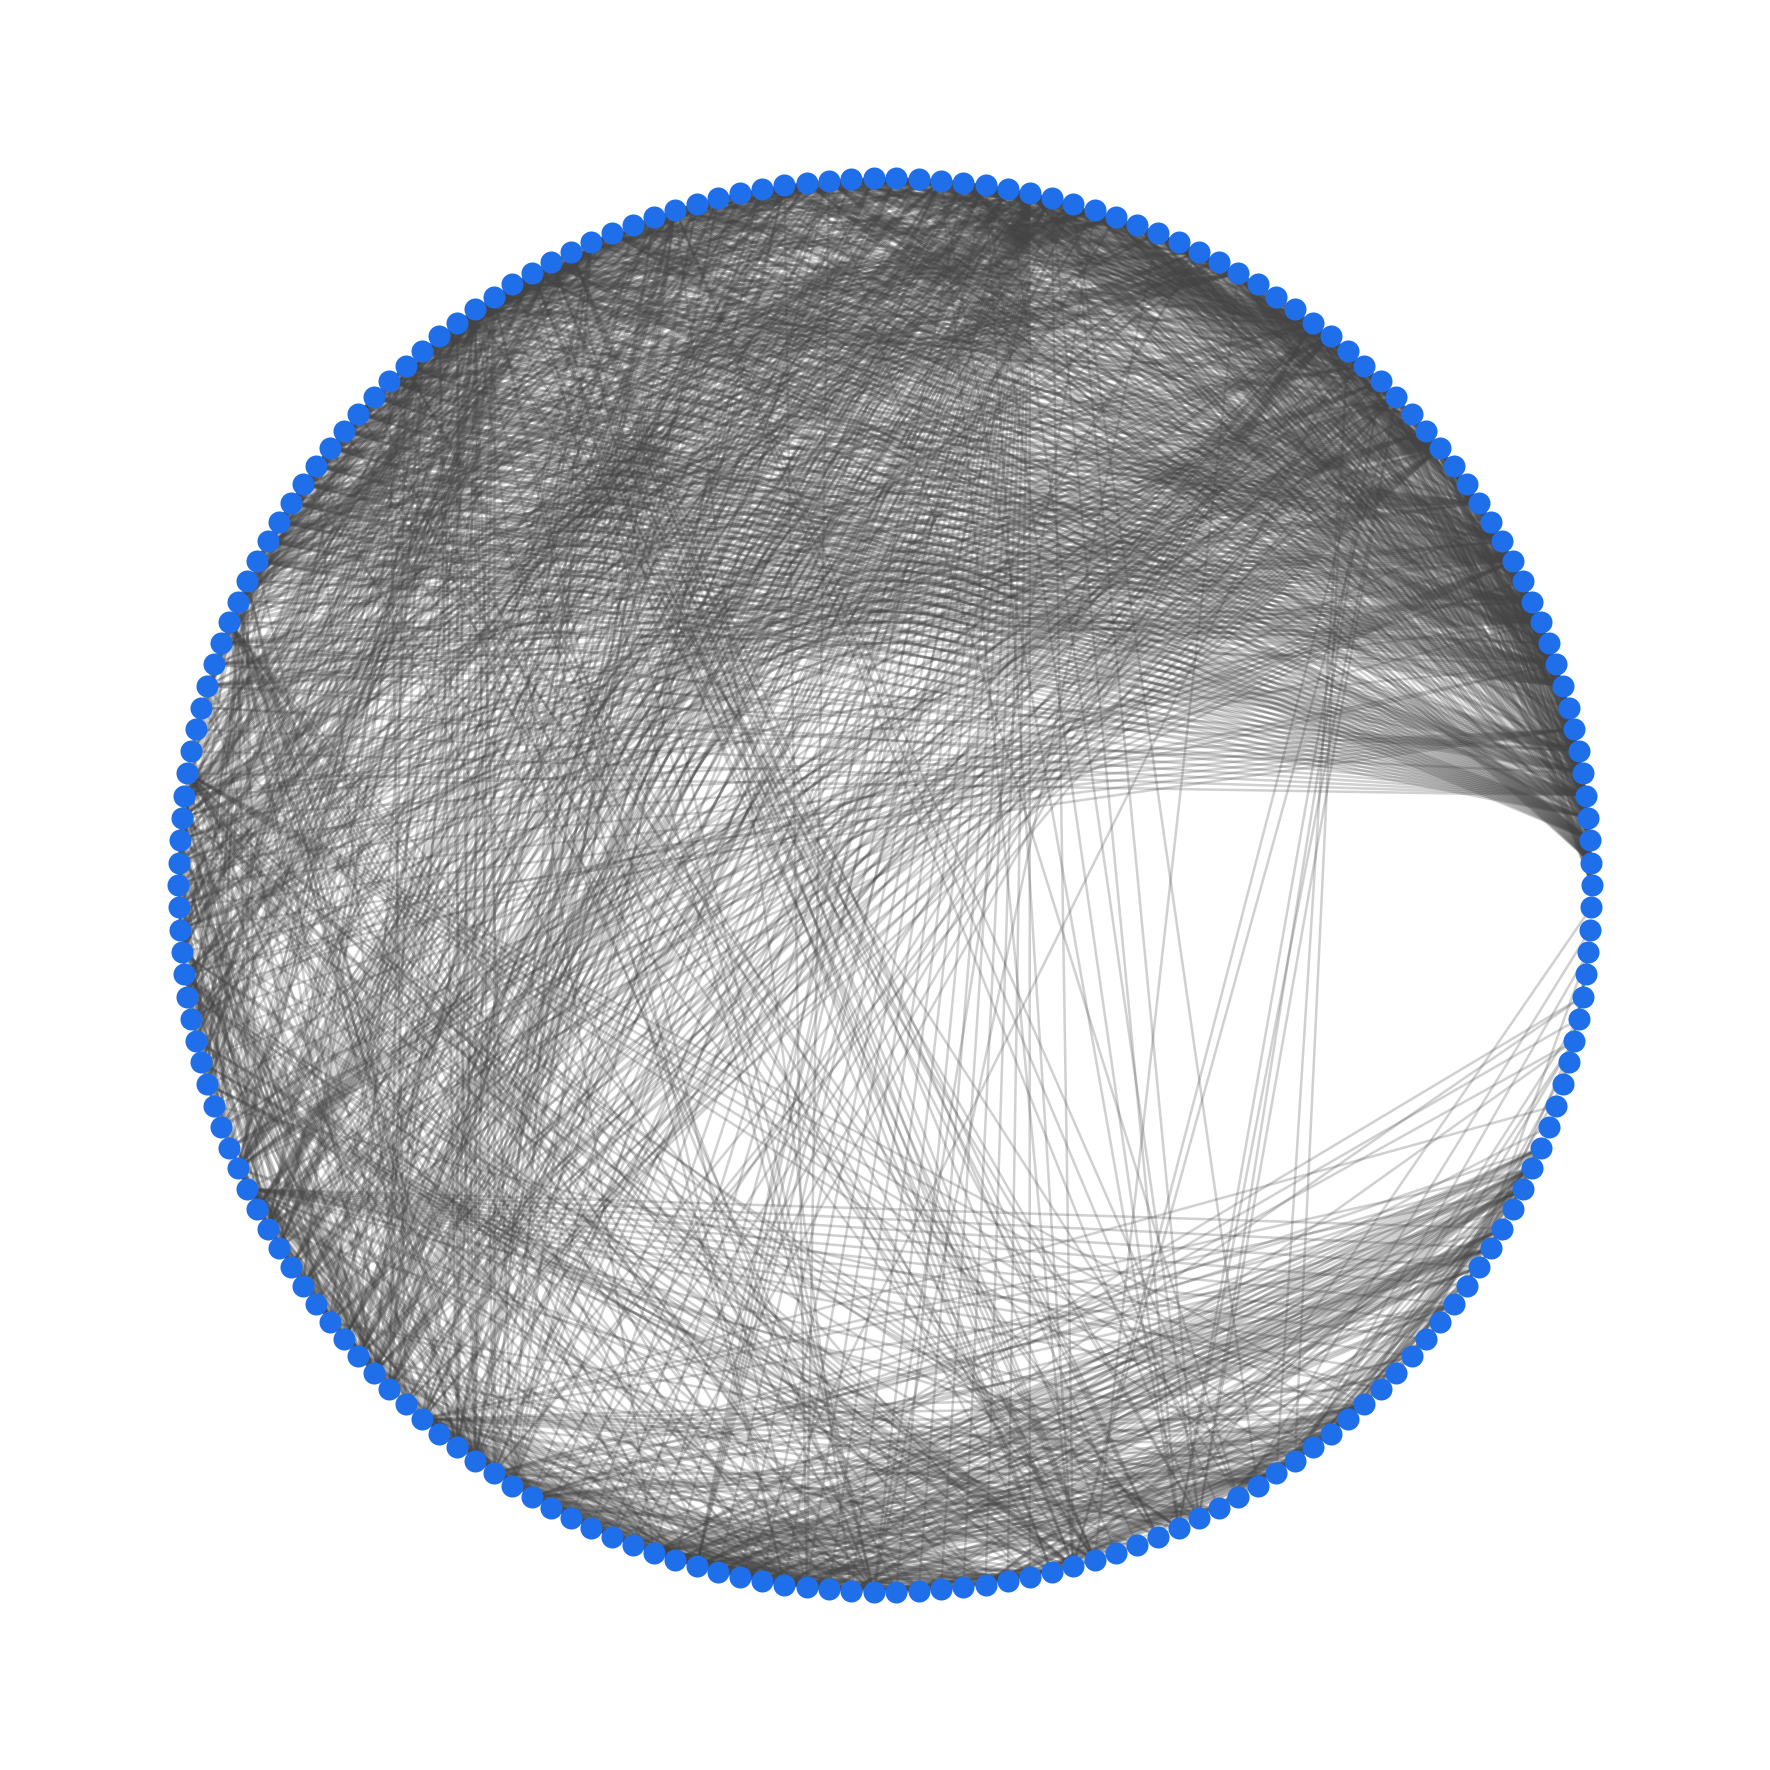
\includegraphics[width=\linewidth]{jazz_circular.png}
\caption{Jazz}
\end{subfigure}
\hfill
\begin{subfigure}[t]{0.30\textwidth}
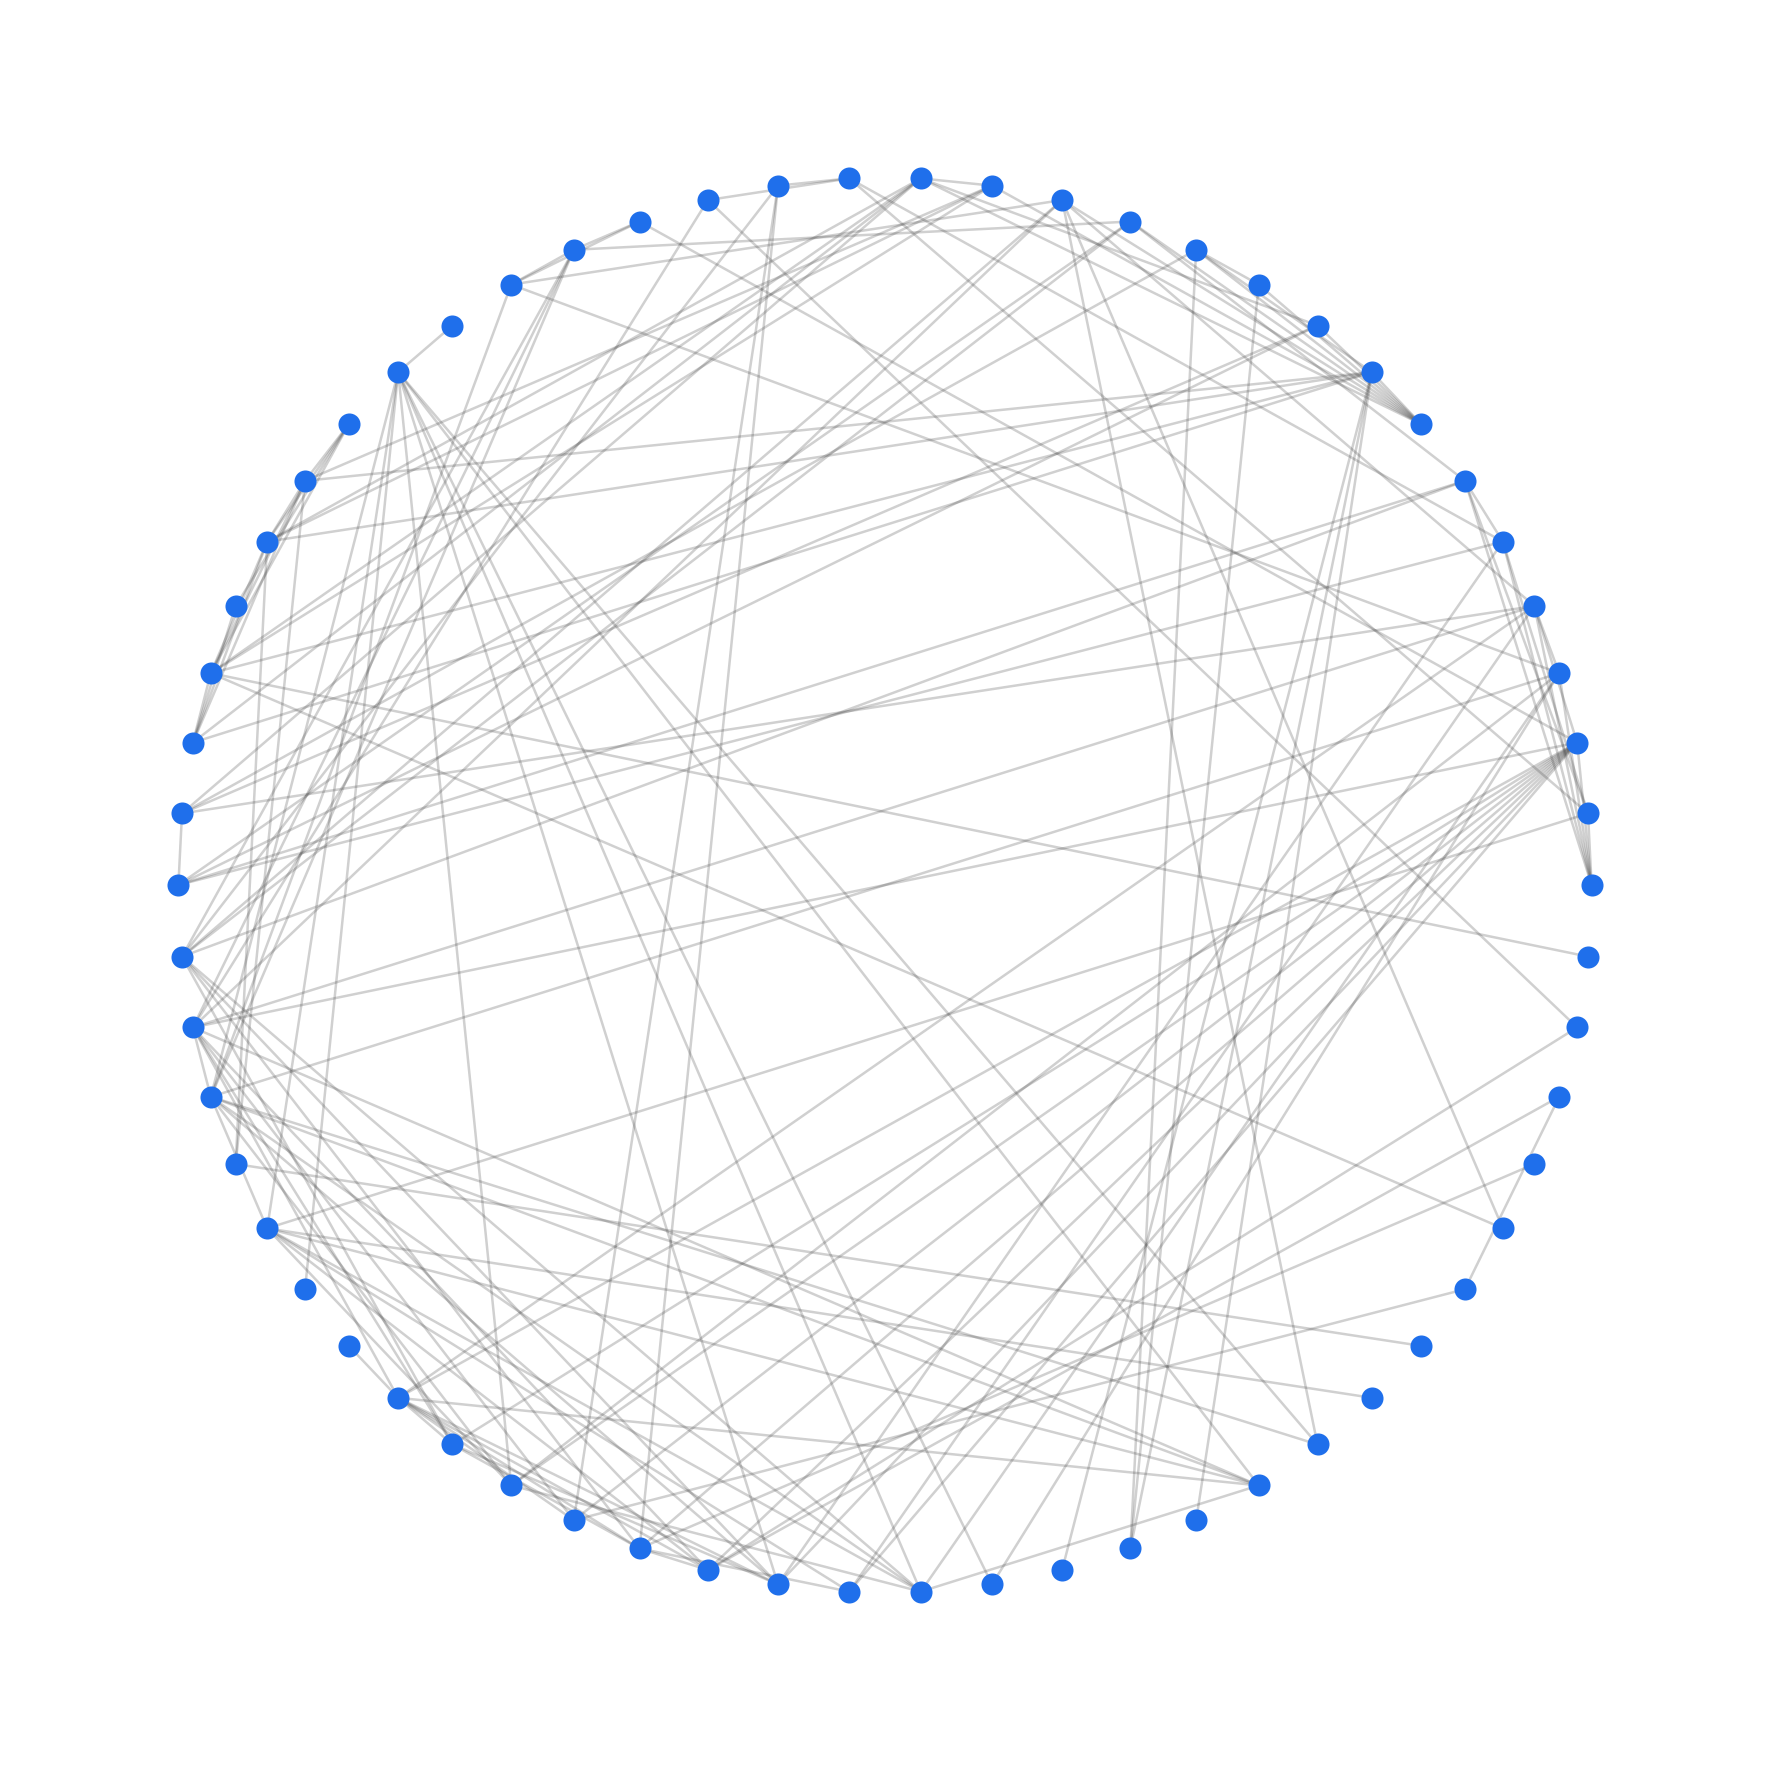
\includegraphics[width=\linewidth]{dolphins_circular.png}
\caption{Dolphins}
\end{subfigure}
\hfill
\begin{subfigure}[t]{0.30\textwidth}
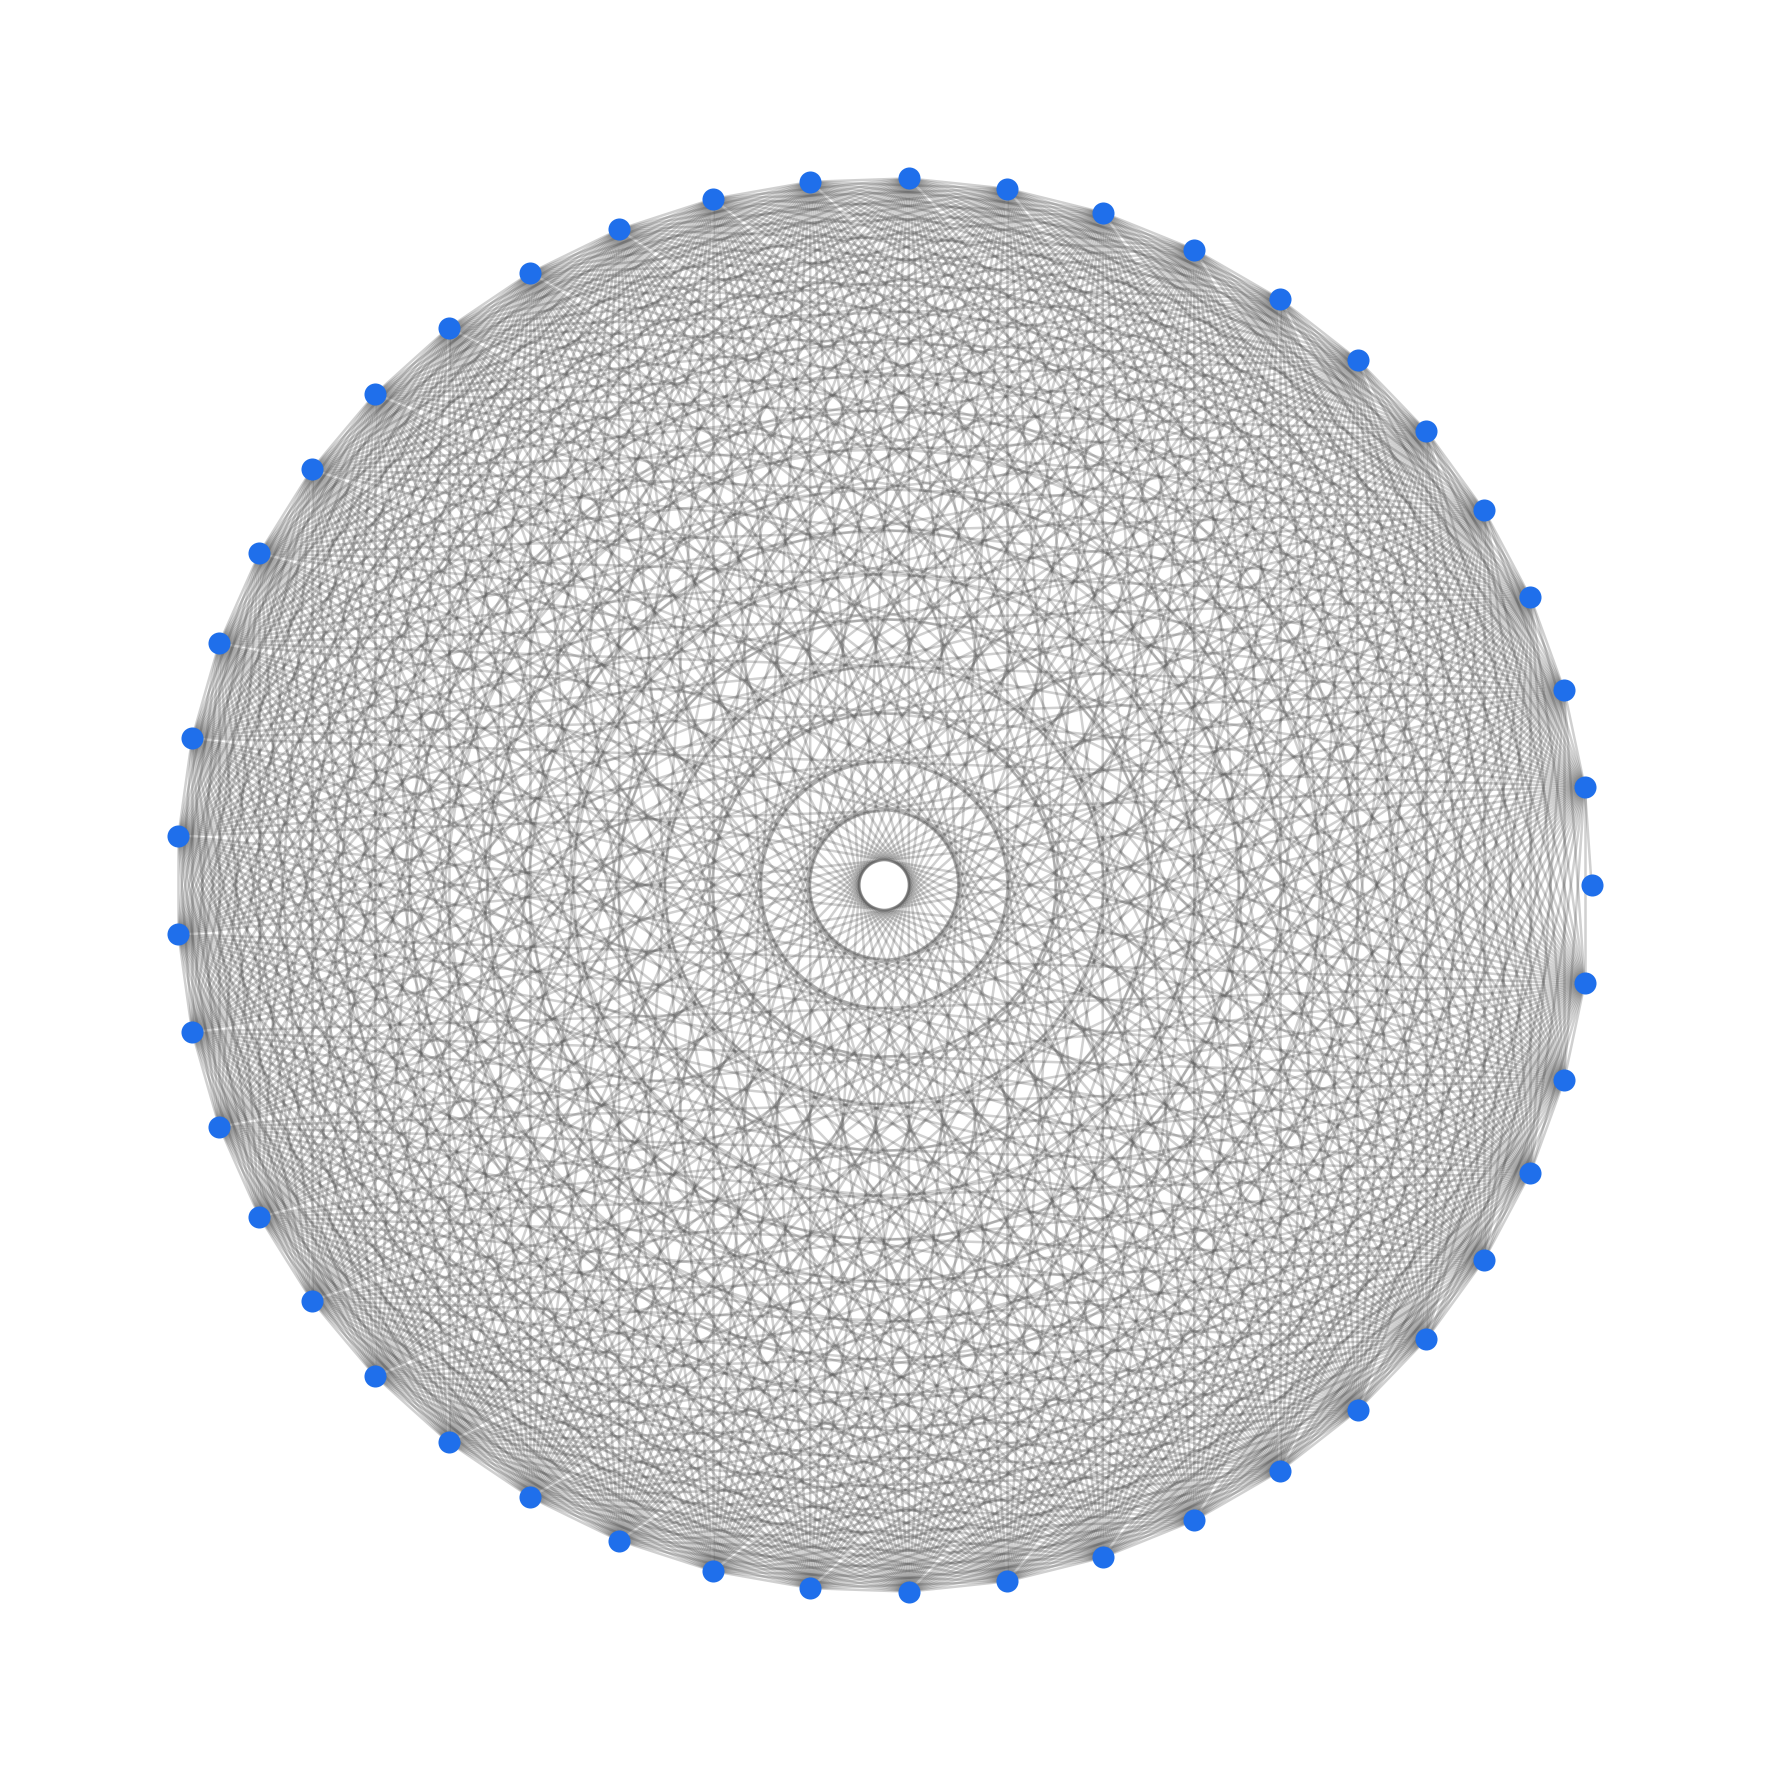
\includegraphics[width=\linewidth]{baseball_circular.png}
\caption{Baseball}
\end{subfigure}
\hfill
\begin{subfigure}[t]{0.30\textwidth}
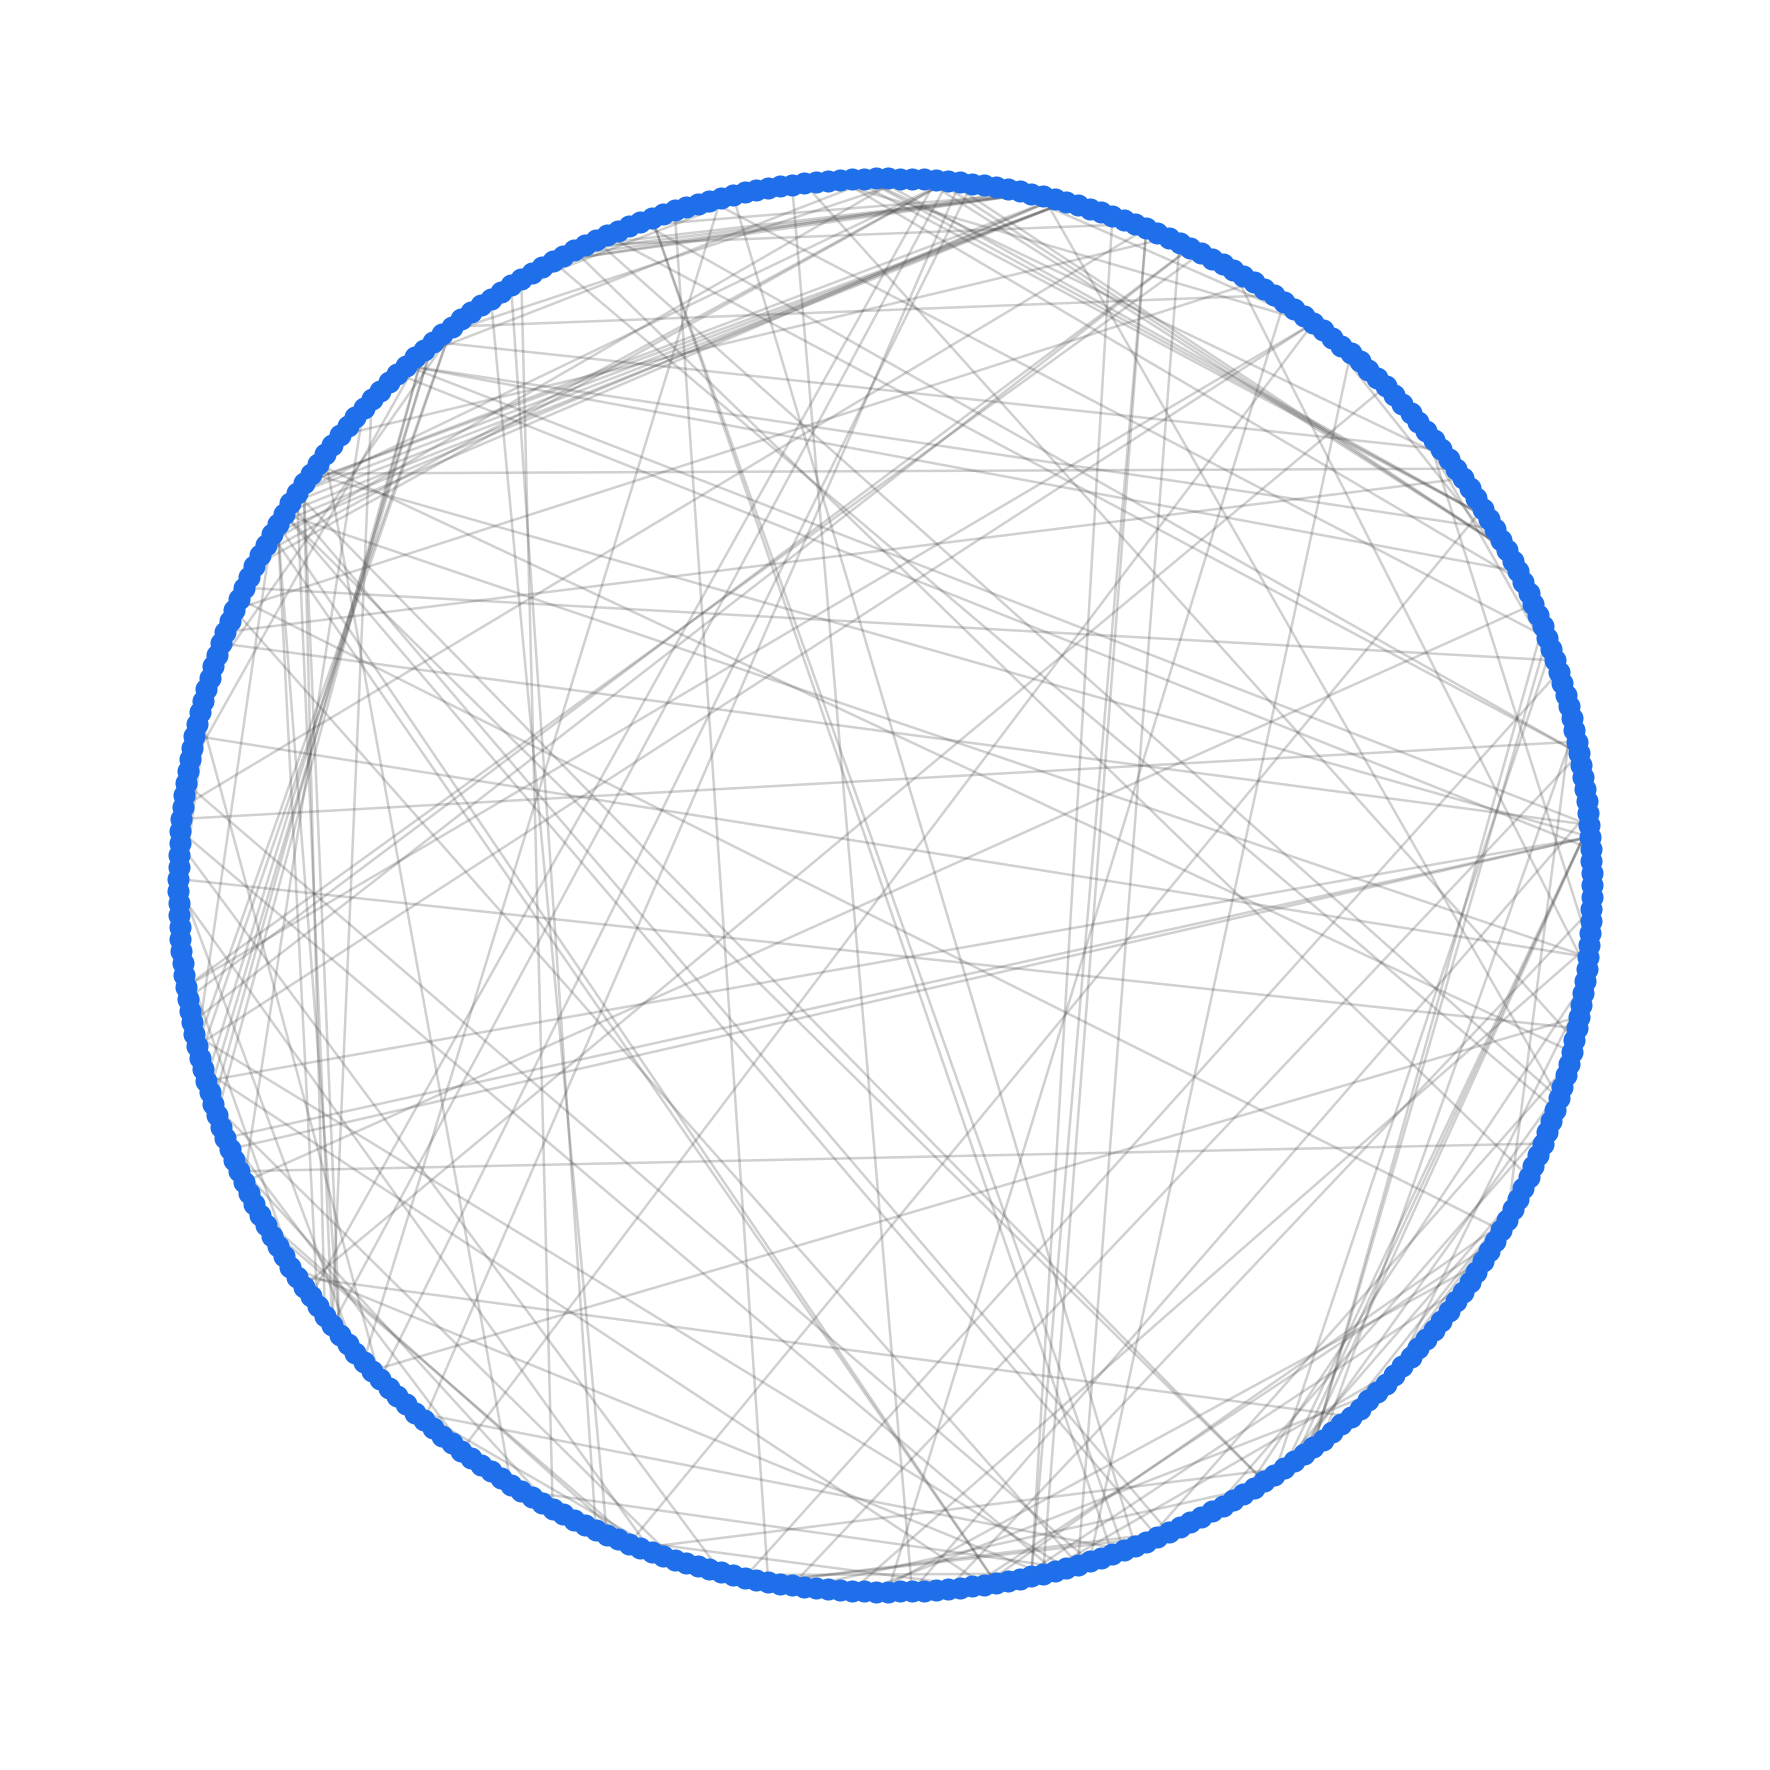
\includegraphics[width=\linewidth]{transport_circular.png}
\caption{Transport}
\end{subfigure}
\caption{Circular layouts of the four benchmark networks. Density and
clustering fall sharply from the near-complete Baseball graph and the
dense Jazz graph to the sparse Dolphins social network and the near-tree
Transport network.}
\label{fig:circular}
\end{figure}

\subsection{Jazz Musicians Network}
\label{sec:net-jazz}
The Jazz network~\cite{gleiser2003jazz} captures collaborations between jazz
musicians; its largest connected component has $198$ nodes and $2742$ edges,
making it a dense, highly clustered medium-scale graph ($\langle
k\rangle=27.7$, $C=0.618$). \Cref{fig:jazz} shows the static (solid) and
iterative (dashed) $R_{gc}(\rho)$ curves for the three metrics. For both
betweenness-based metrics the iterative curve falls earlier and steeper than its
static counterpart: in such a dense graph each removal strongly rewires the local
geodesic structure that LLBCe and LLBMEe1 depend on, so recomputation pays off,
and LLBMEe1 improves more than any other network-metric combination in this
study. For LDC the two curves nearly coincide and the iterative variant is
slightly worse. On a graph this dense the degree-product ordering is already
near-optimal, so recomputation just reshuffles edges of near-equal structural
value.

\begin{figure}[t]
\centering
\begin{subfigure}[t]{0.32\textwidth}
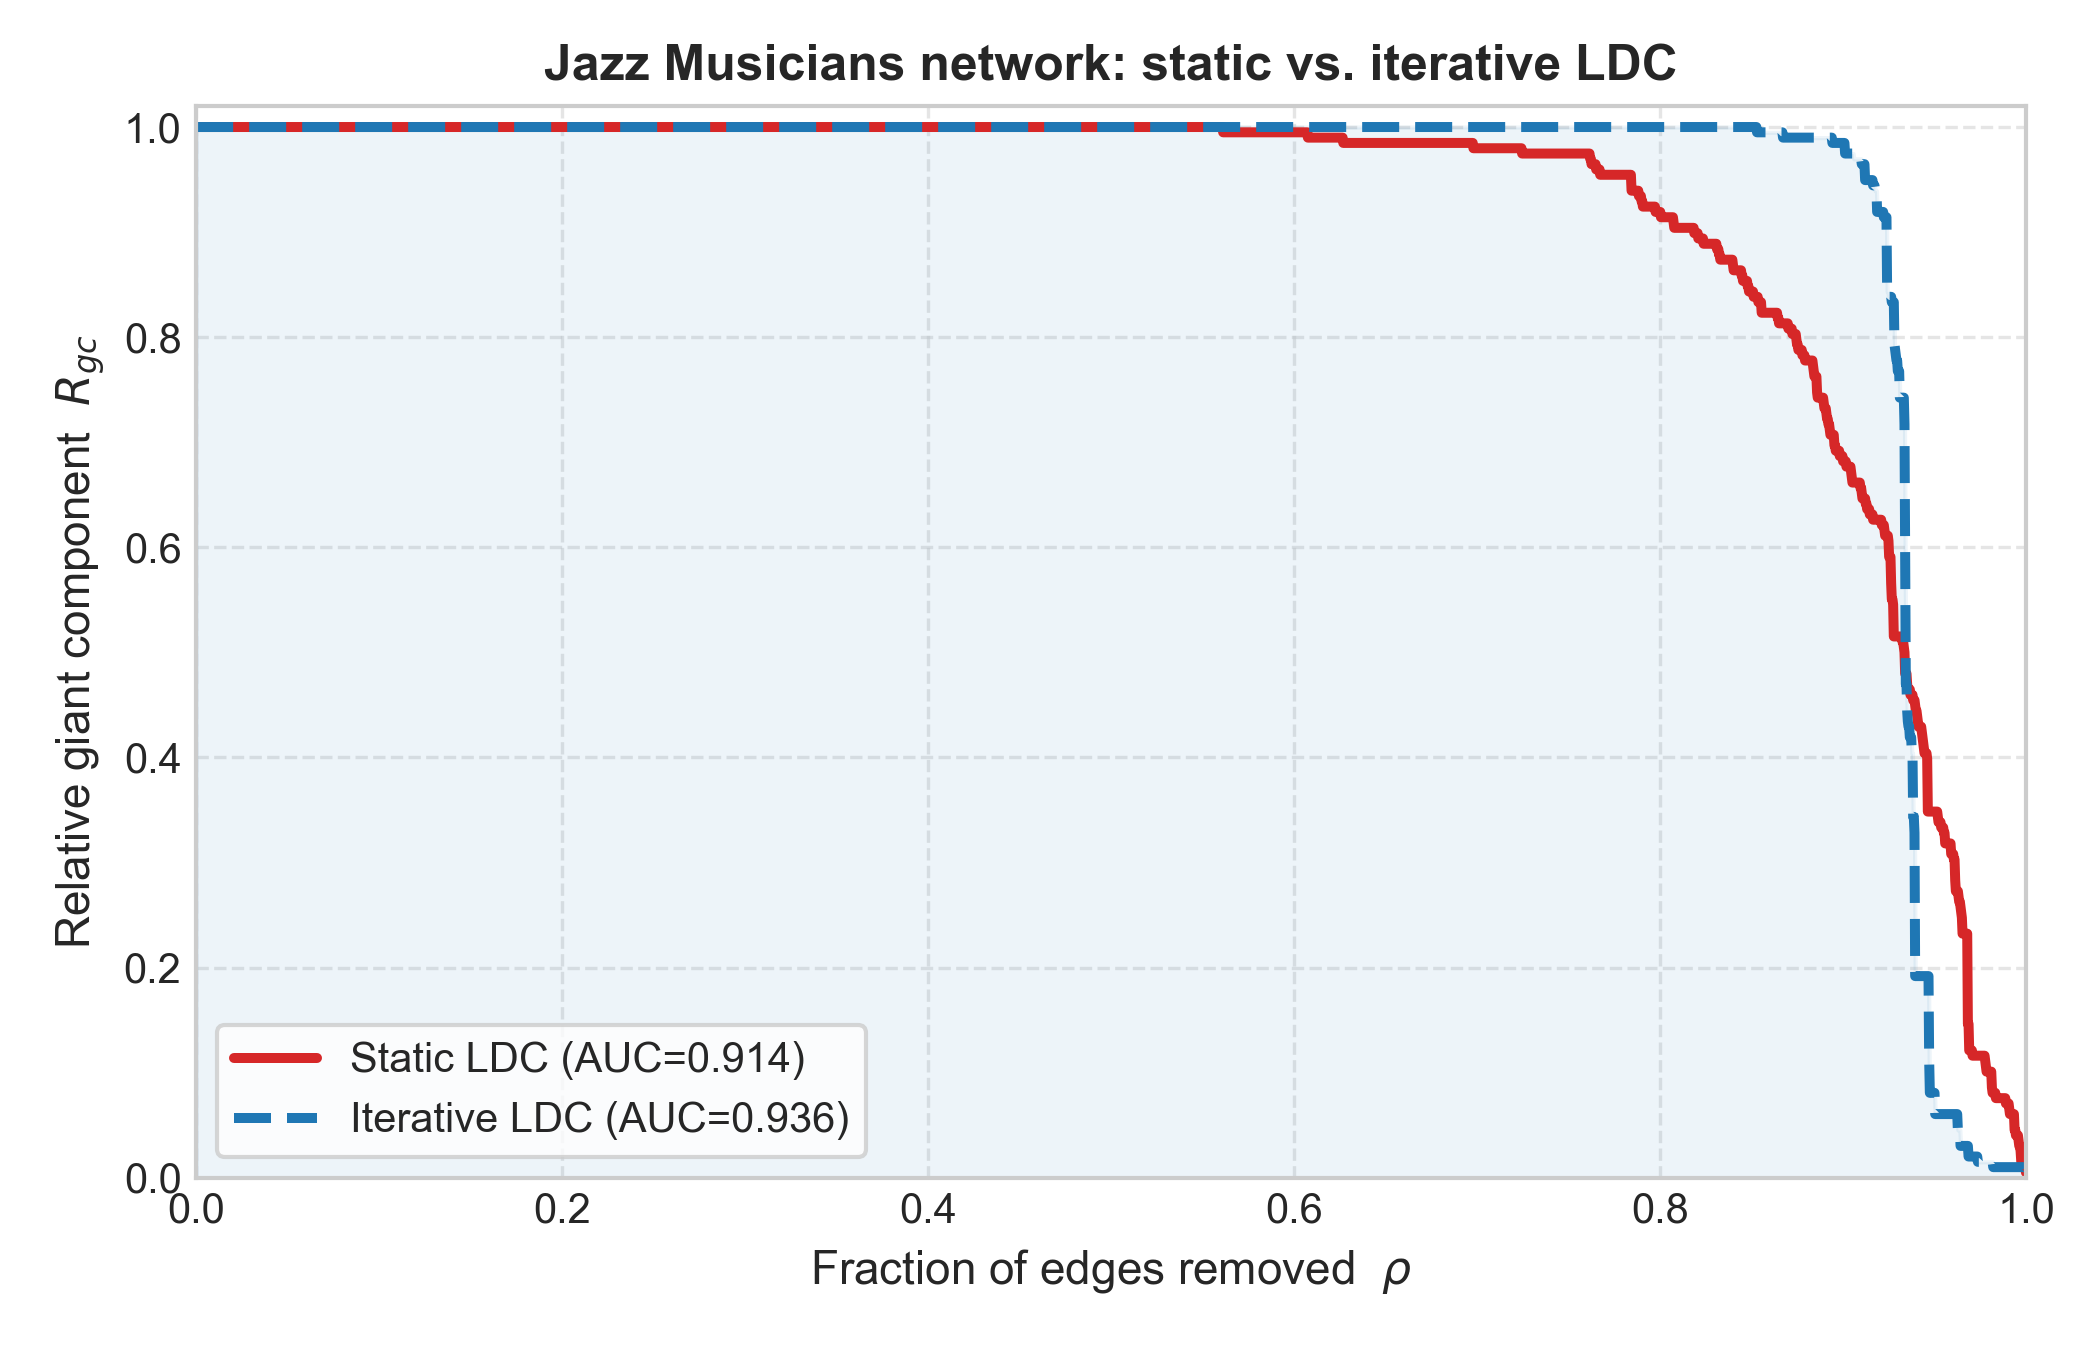
\includegraphics[width=\linewidth]{jazz_LDC.png}
\caption{LDC}
\end{subfigure}
\hfill
\begin{subfigure}[t]{0.32\textwidth}
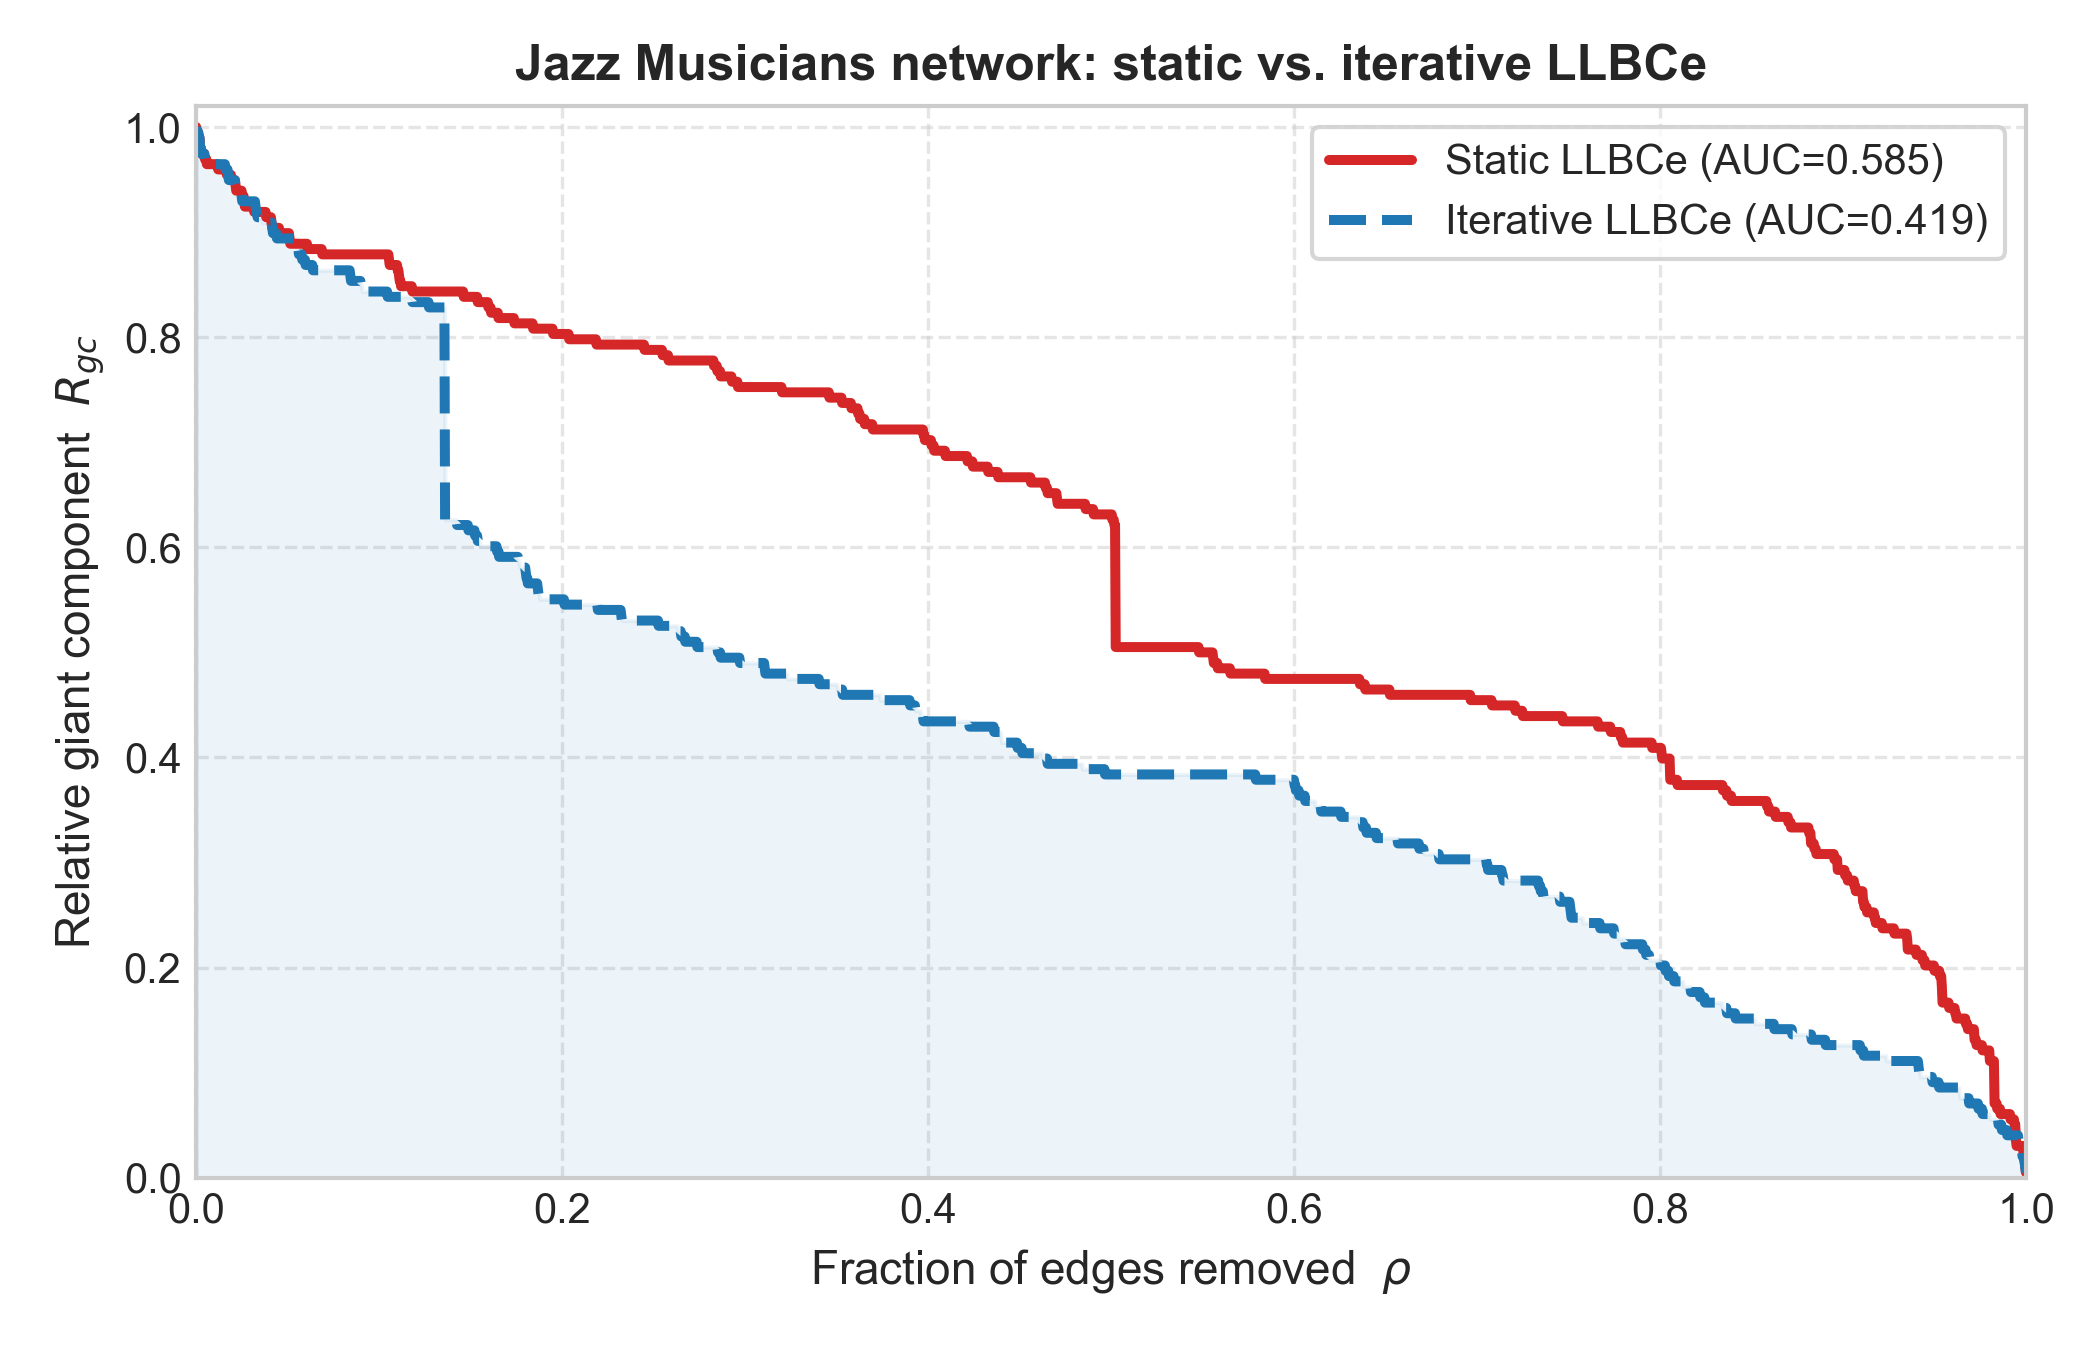
\includegraphics[width=\linewidth]{jazz_LLBCe.png}
\caption{LLBCe}
\end{subfigure}
\hfill
\begin{subfigure}[t]{0.32\textwidth}
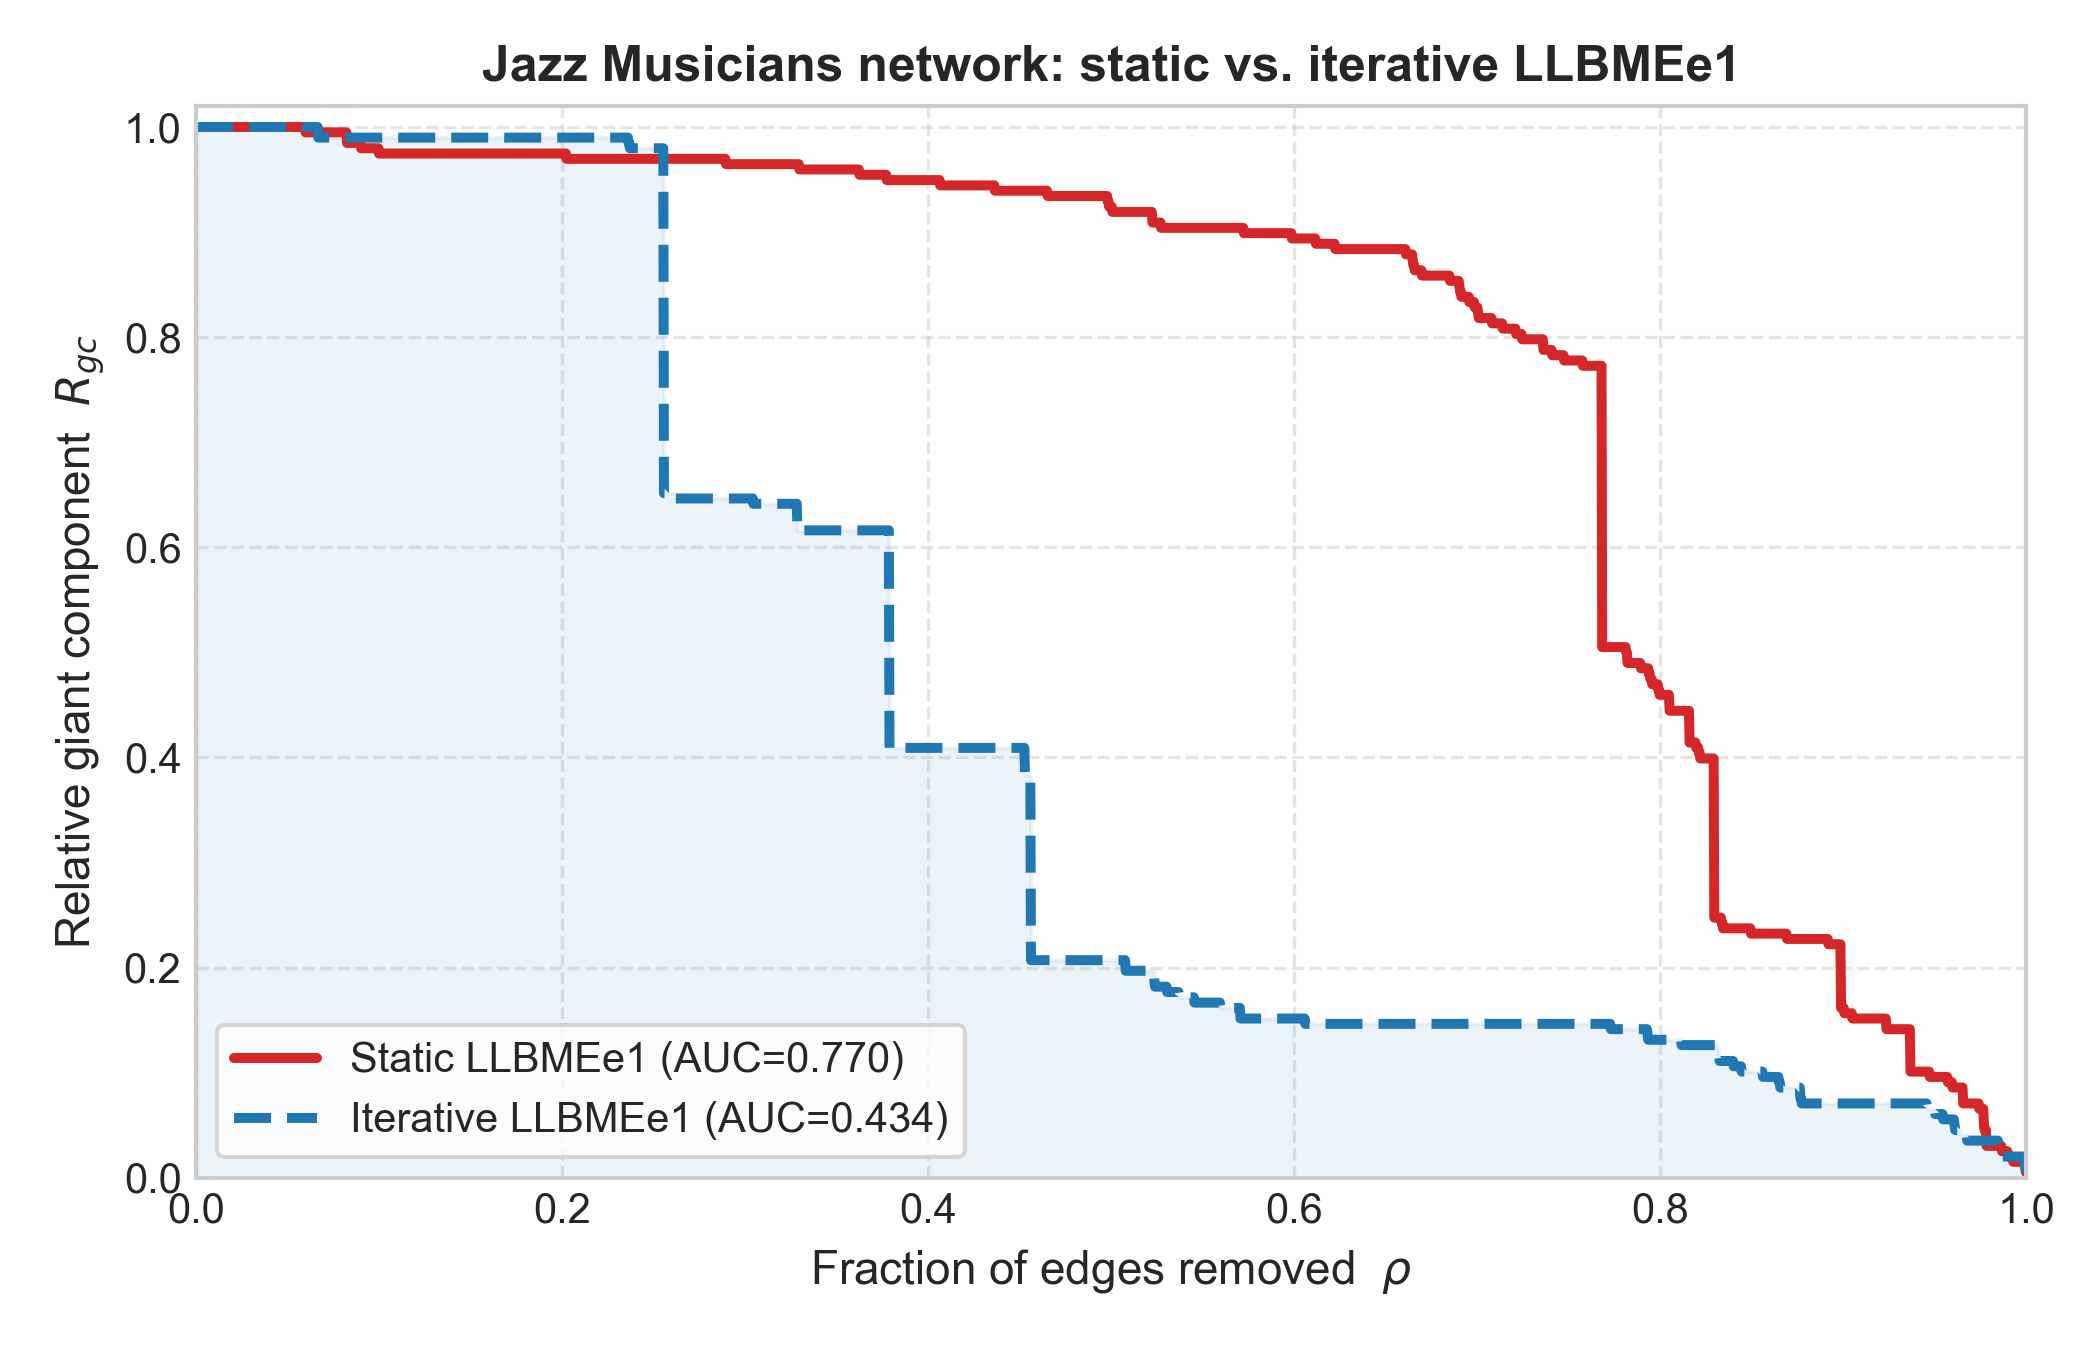
\includegraphics[width=\linewidth]{jazz_LLBMEe1.png}
\caption{LLBMEe1}
\end{subfigure}
\caption{Static (solid) vs.\ iterative (dashed) dismantling curves for the
\textbf{Jazz} network. Iteration sharpens both betweenness-based metrics
strongly but does not help the degree product.}
\label{fig:jazz}
\end{figure}

\subsection{Dolphins Social Network}
\label{sec:net-dolphins}
The Dolphins network~\cite{lusseau2003dolphins} records $159$ associations among
$62$ bottlenose dolphins of Doubtful Sound, New Zealand, and is a small, sparse
social graph with a pronounced two-community structure ($\langle k\rangle=5.1$,
$C=0.259$). \Cref{fig:dolphins} shows its decomposition curves. Here iteration
helps \emph{all three} metrics: both betweenness-based metrics again improve
substantially, and even LDC benefits modestly, because in a sparse community
graph the degree product does become stale as the few inter-community links are
exposed by successive removals. The iterative curves drop earlier, confirming
that the adaptive ranking captures the bridging edges between the two
communities more reliably than the static one.

\begin{figure}[t]
\centering
\begin{subfigure}[t]{0.32\textwidth}
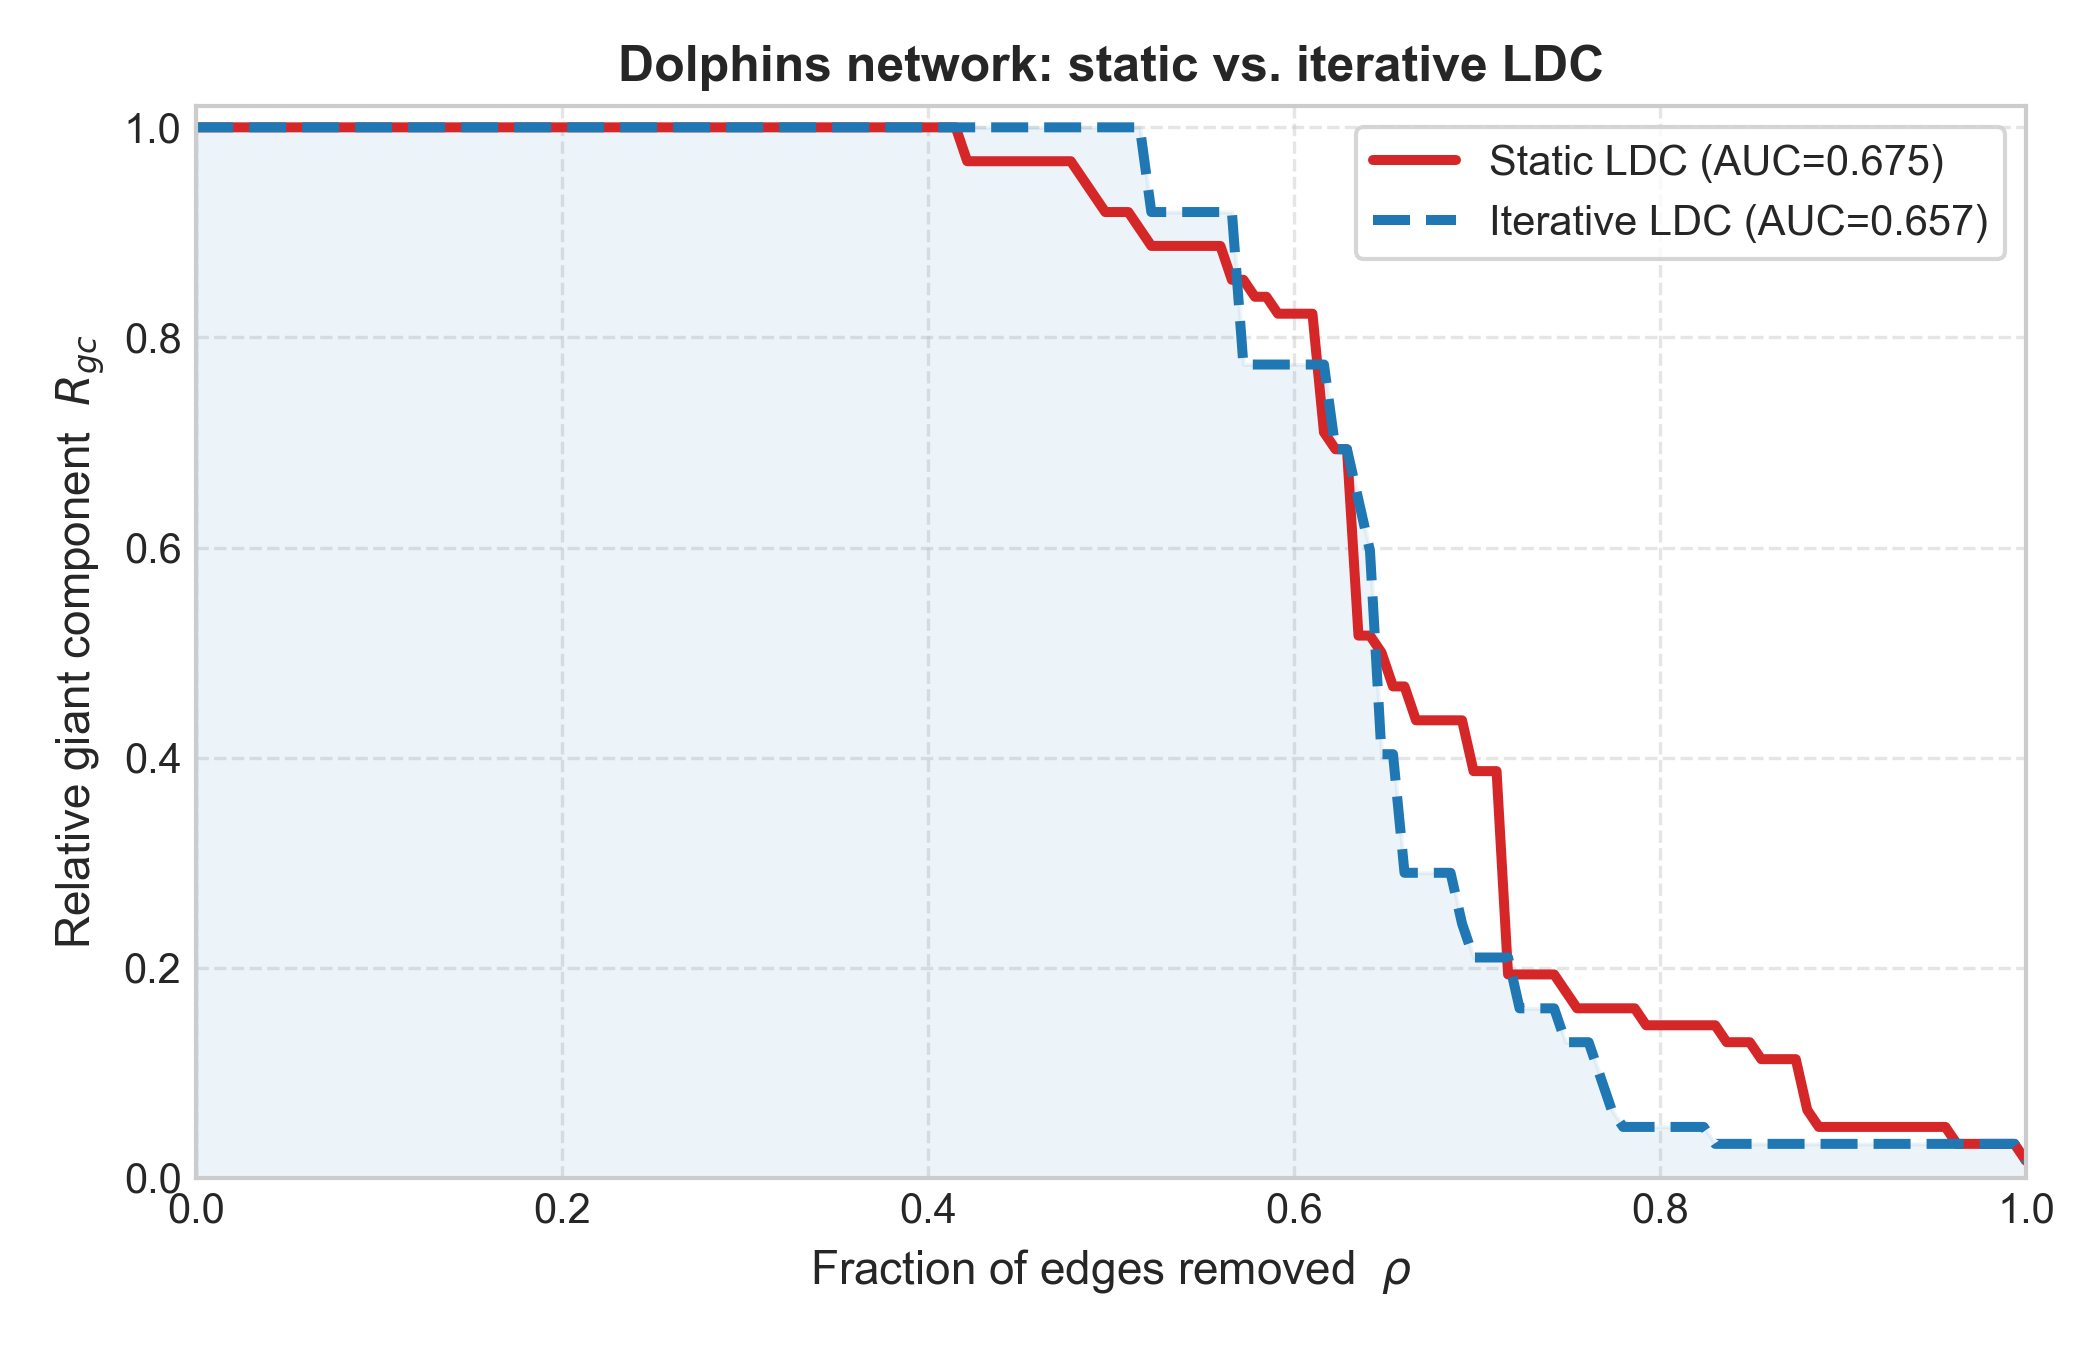
\includegraphics[width=\linewidth]{dolphins_LDC.png}
\caption{LDC}
\end{subfigure}
\hfill
\begin{subfigure}[t]{0.32\textwidth}
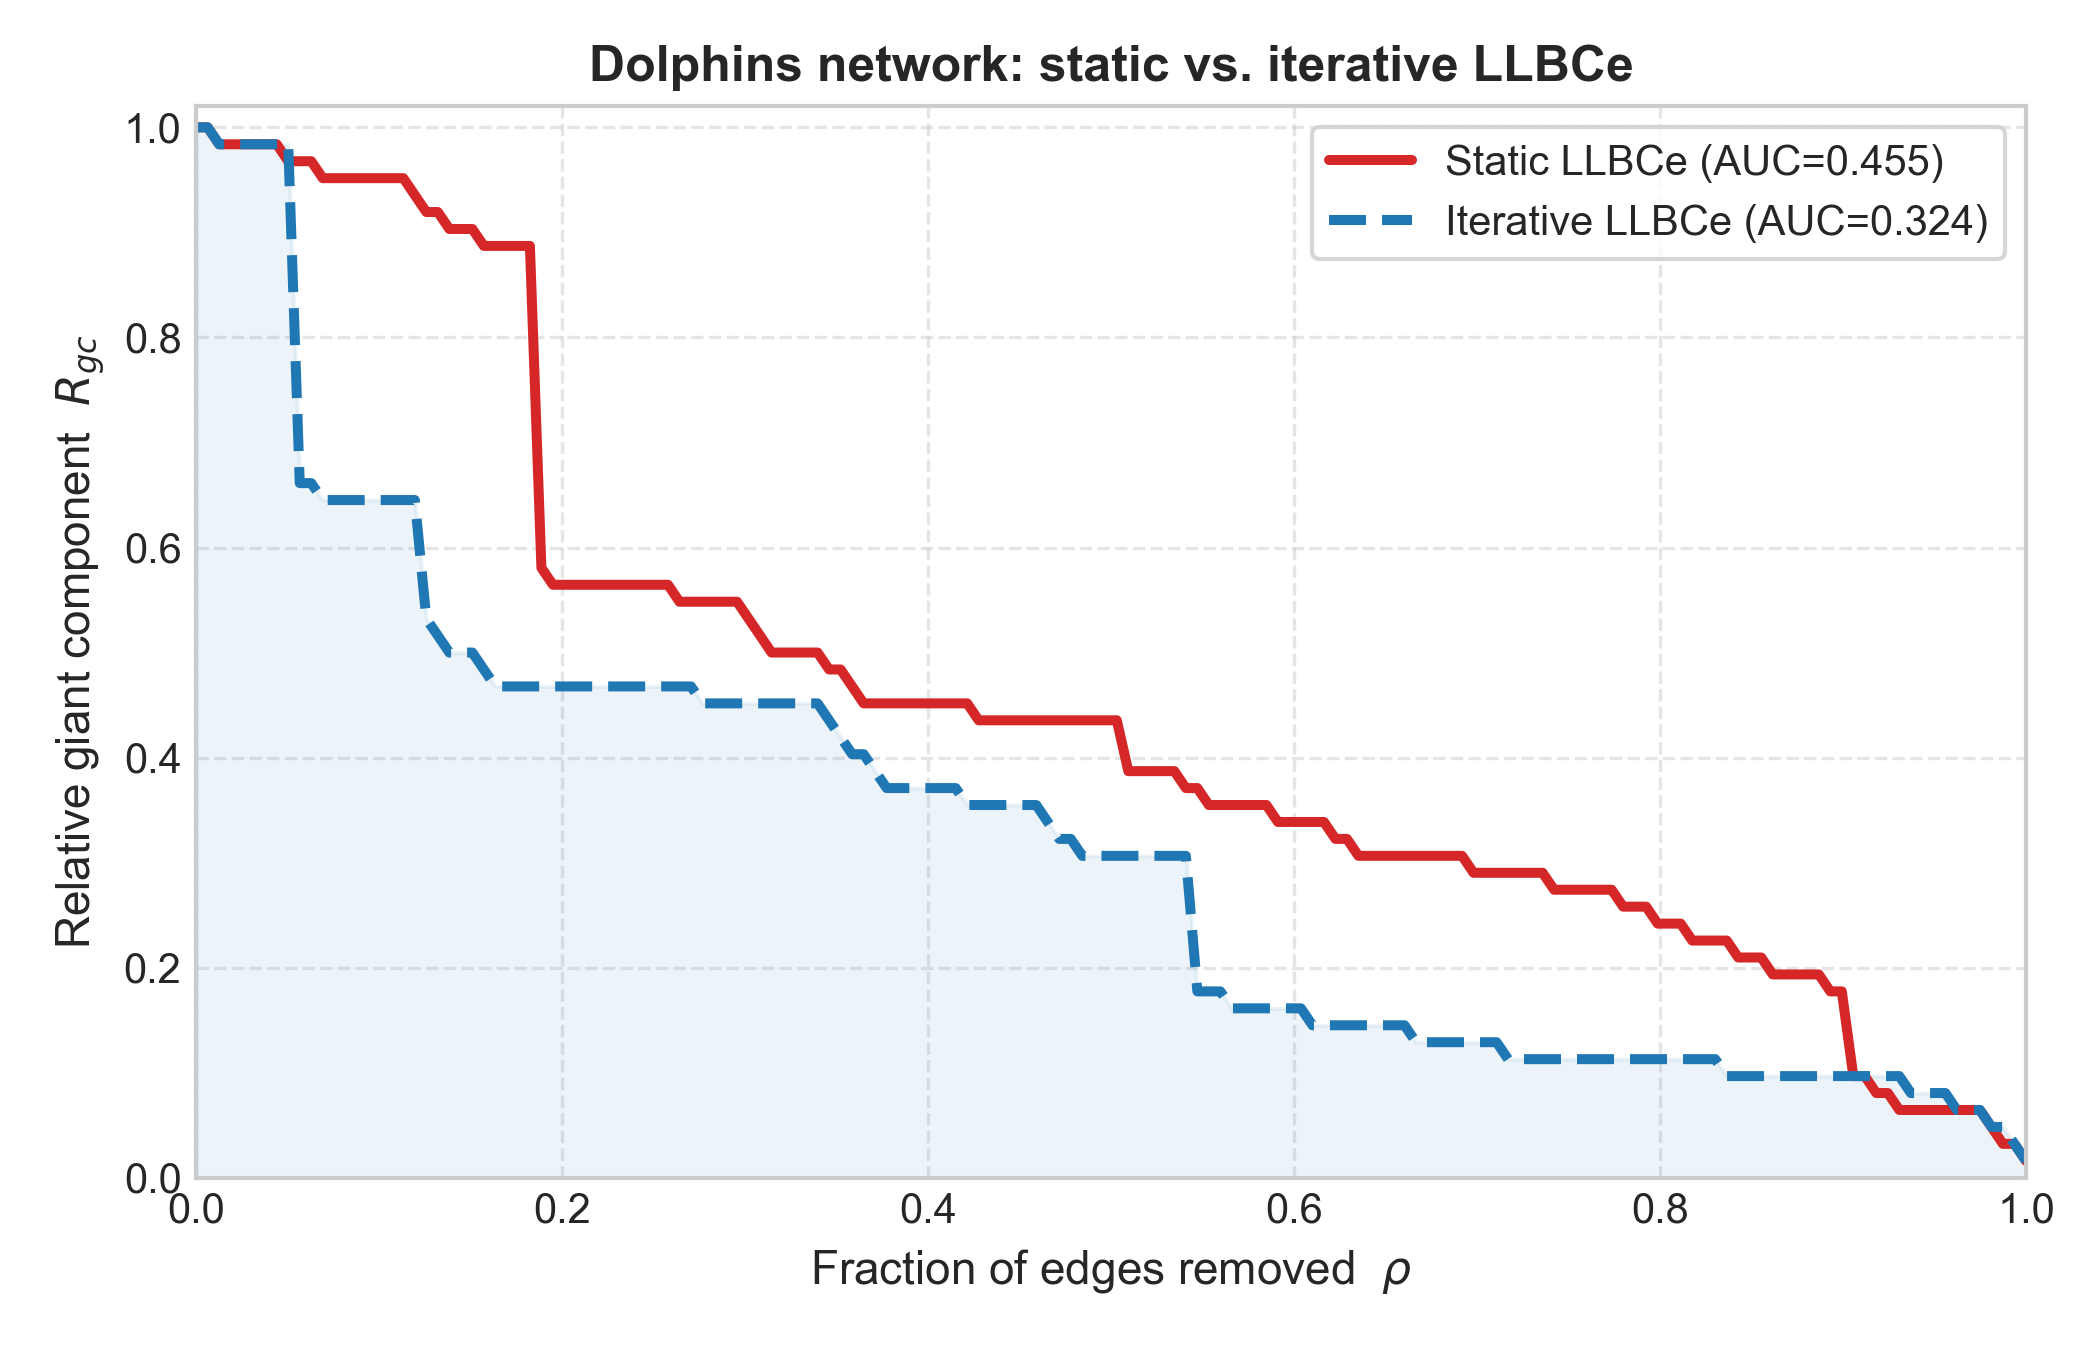
\includegraphics[width=\linewidth]{dolphins_LLBCe.png}
\caption{LLBCe}
\end{subfigure}
\hfill
\begin{subfigure}[t]{0.32\textwidth}
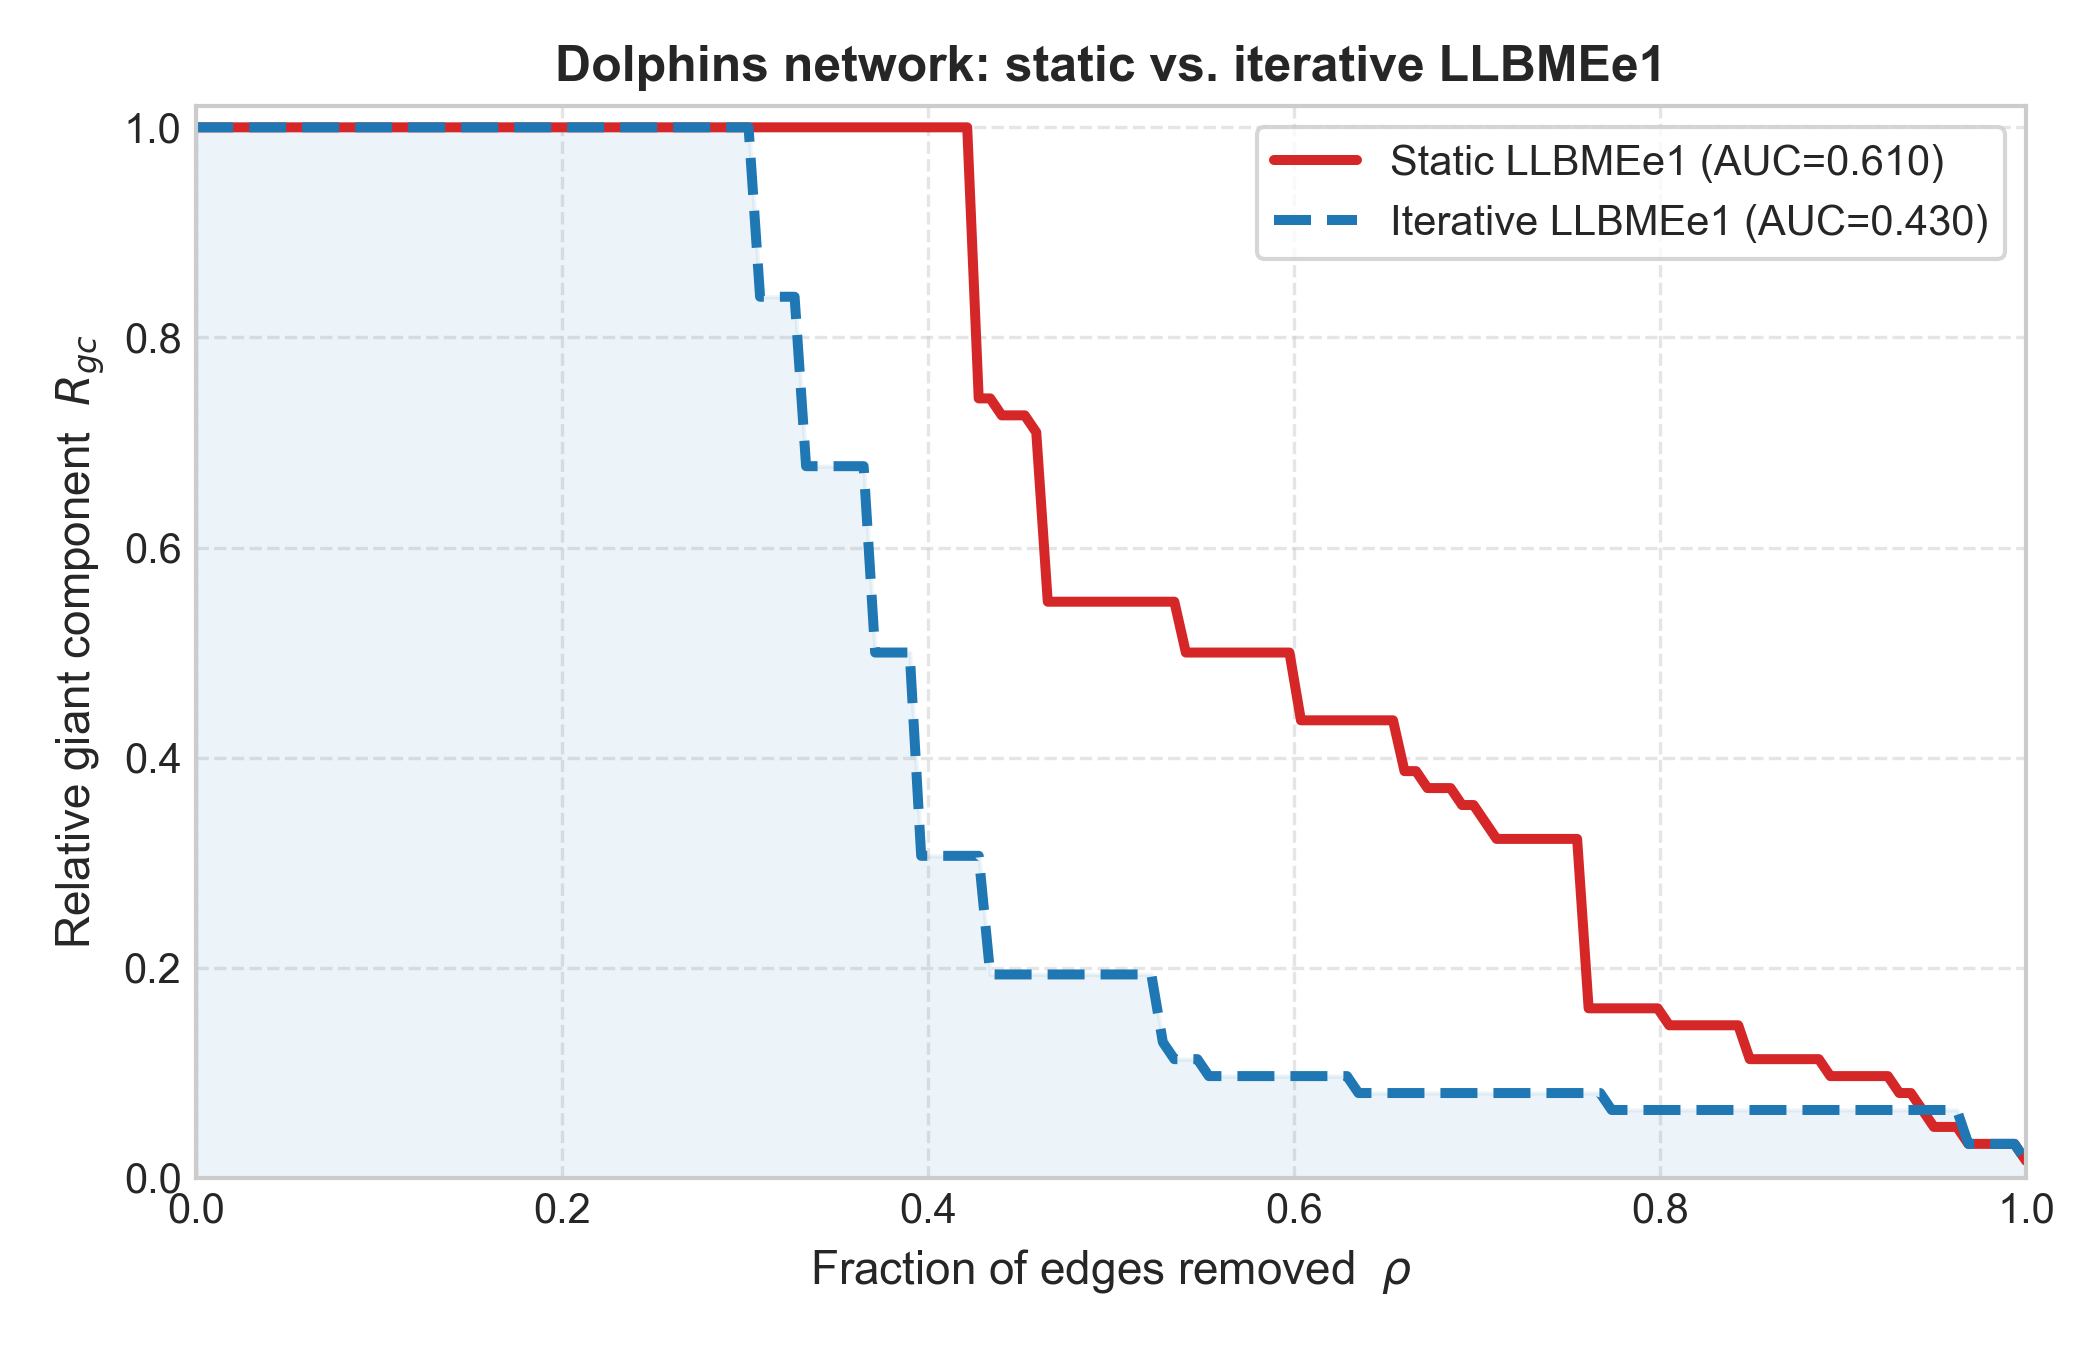
\includegraphics[width=\linewidth]{dolphins_LLBMEe1.png}
\caption{LLBMEe1}
\end{subfigure}
\caption{Static (solid) vs.\ iterative (dashed) dismantling curves for the
\textbf{Dolphins} network. All three metrics improve under iteration on this
sparse, two-community graph.}
\label{fig:dolphins}
\end{figure}

\subsection{Baseball Association Network}
\label{sec:net-baseball}
The Baseball network is an exceptionally dense, near-complete association graph
of $45$ nodes and $947$ edges derived from a steroid-distribution case
($C=0.977$, density $0.957$). Because almost every pair of nodes is connected,
the three static metrics produce nearly identical AUC values (all $0.936$):
when the graph is this close to complete, local betweenness, degree product and
mapping entropy all rank edges almost interchangeably. \Cref{fig:baseball} shows
the decomposition. Iteration transforms the two betweenness-based metrics, with
LLBCe and LLBMEe1 each falling from $0.936$ to roughly $0.67$, because
recomputation breaks the static ties and exposes the thin structural backbone
that survives once the redundant edges are stripped away. LDC again resists
iteration on this dense graph and worsens slightly, as it did on Jazz.

\begin{figure}[t]
\centering
\begin{subfigure}[t]{0.32\textwidth}
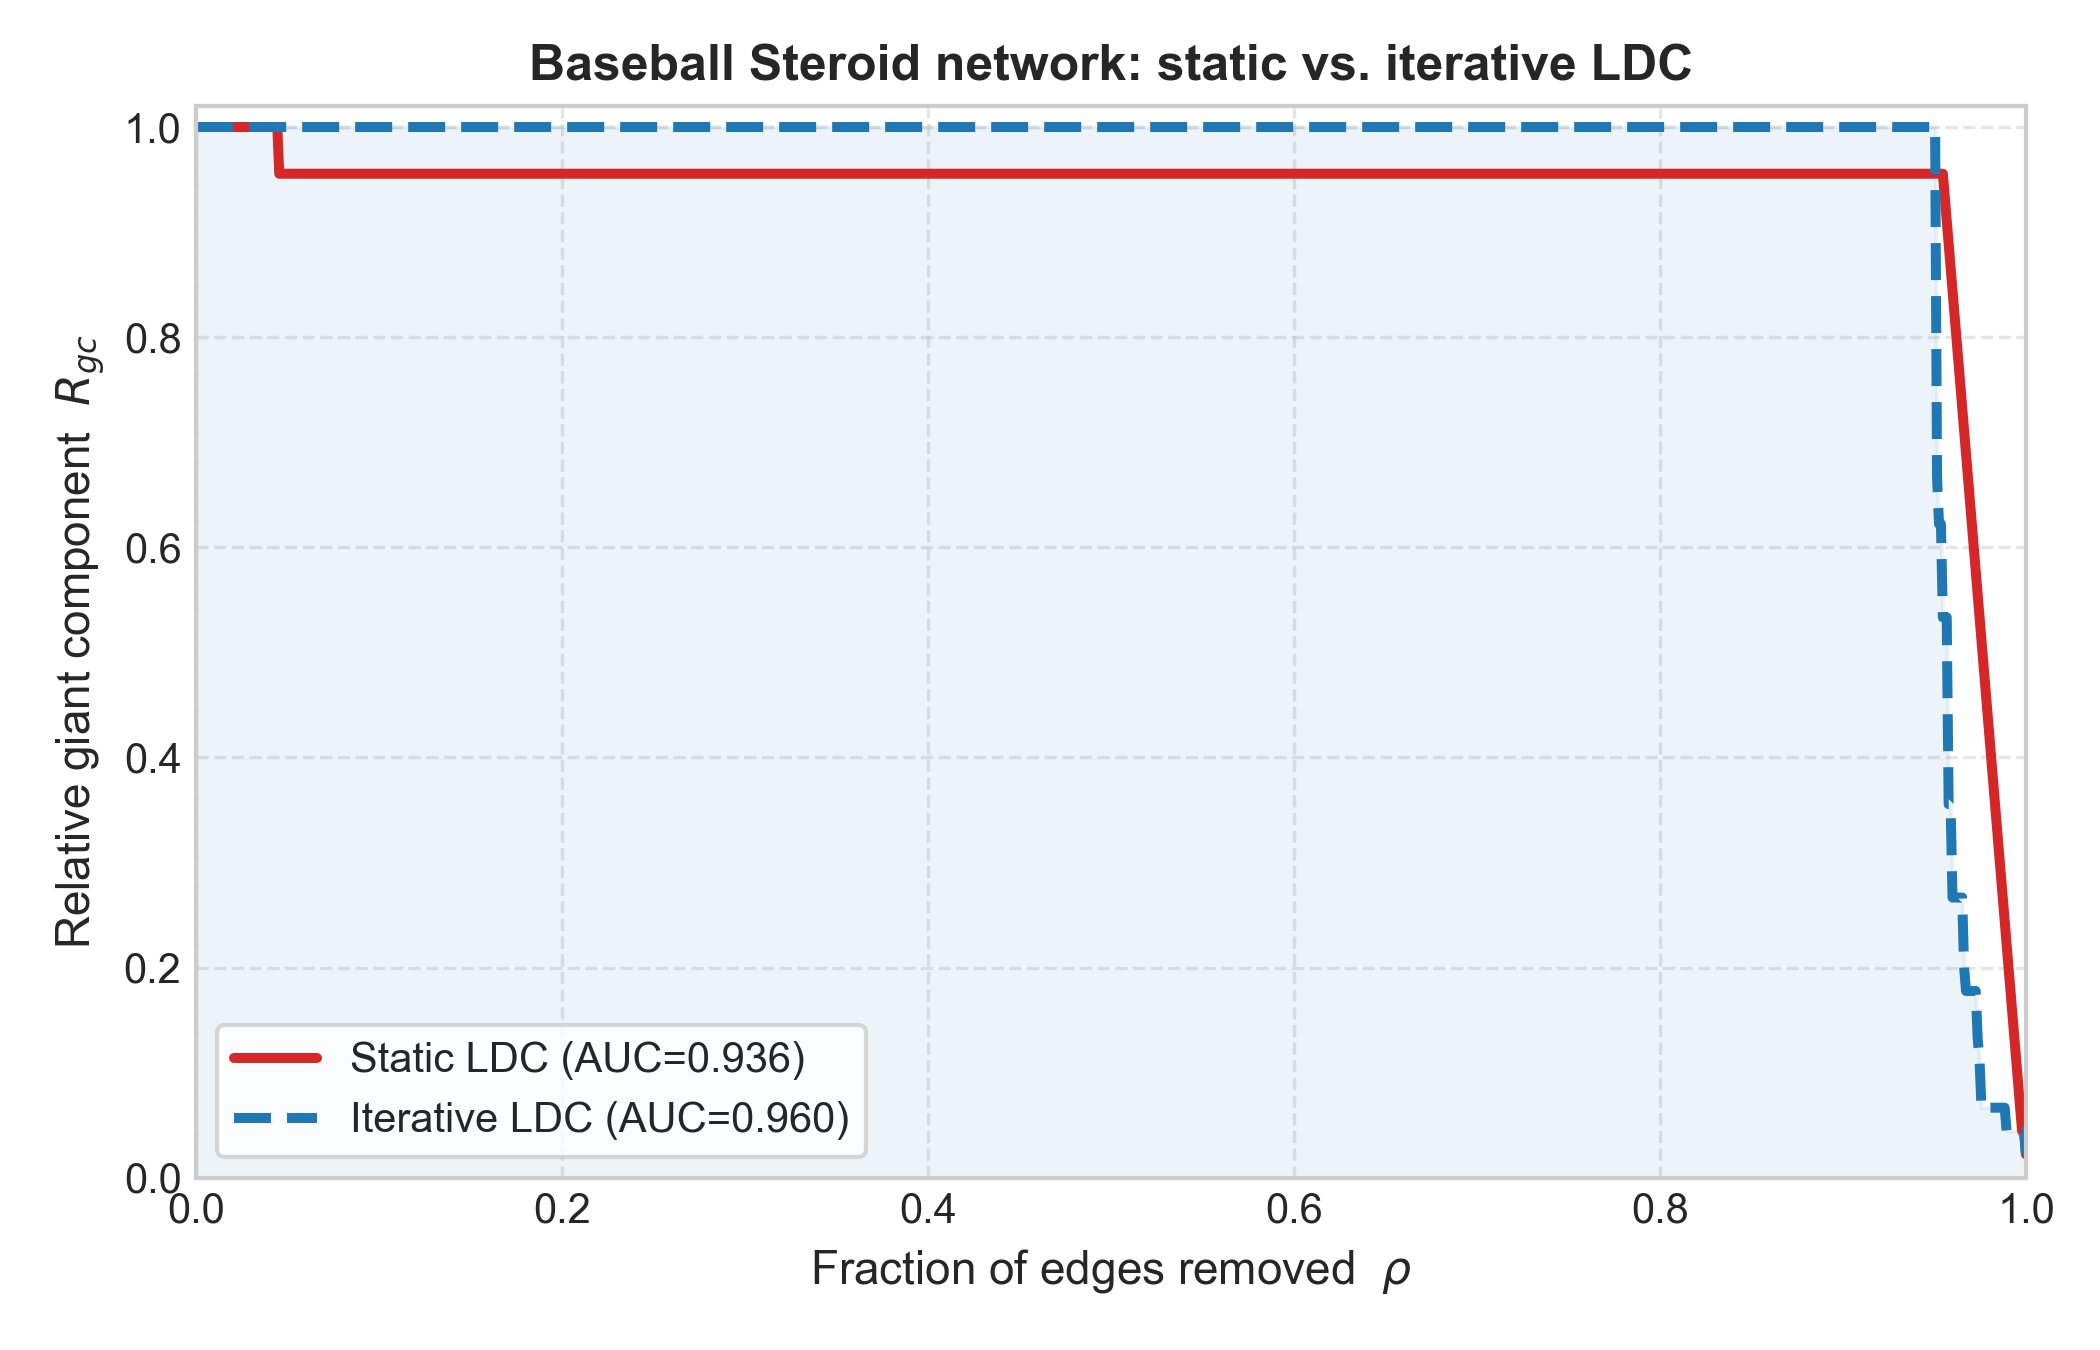
\includegraphics[width=\linewidth]{baseball_LDC.png}
\caption{LDC}
\end{subfigure}
\hfill
\begin{subfigure}[t]{0.32\textwidth}
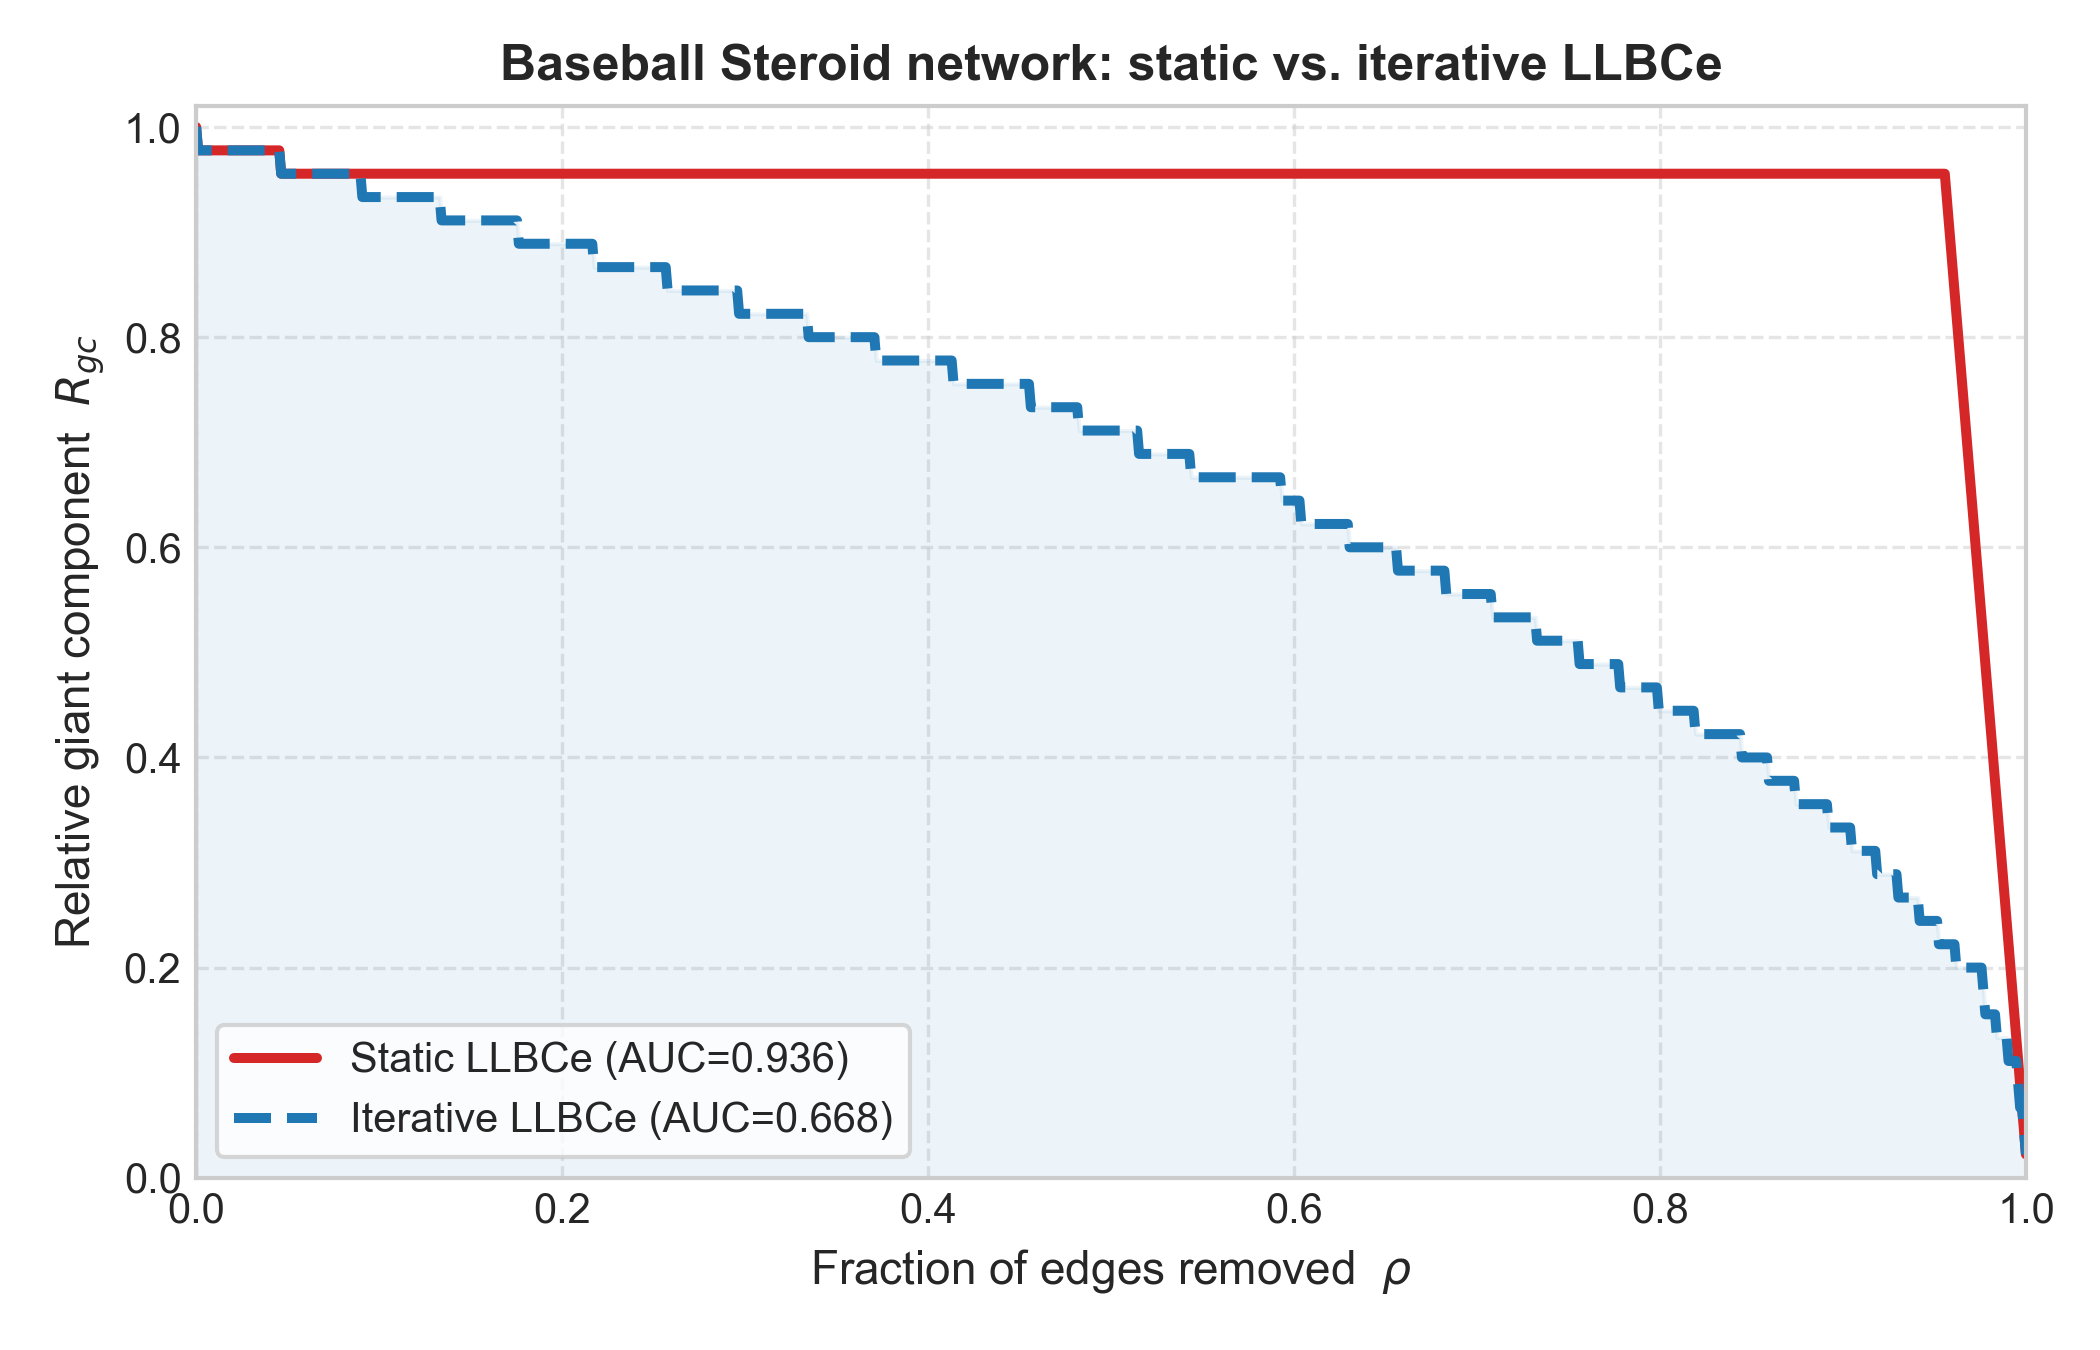
\includegraphics[width=\linewidth]{baseball_LLBCe.png}
\caption{LLBCe}
\end{subfigure}
\hfill
\begin{subfigure}[t]{0.32\textwidth}
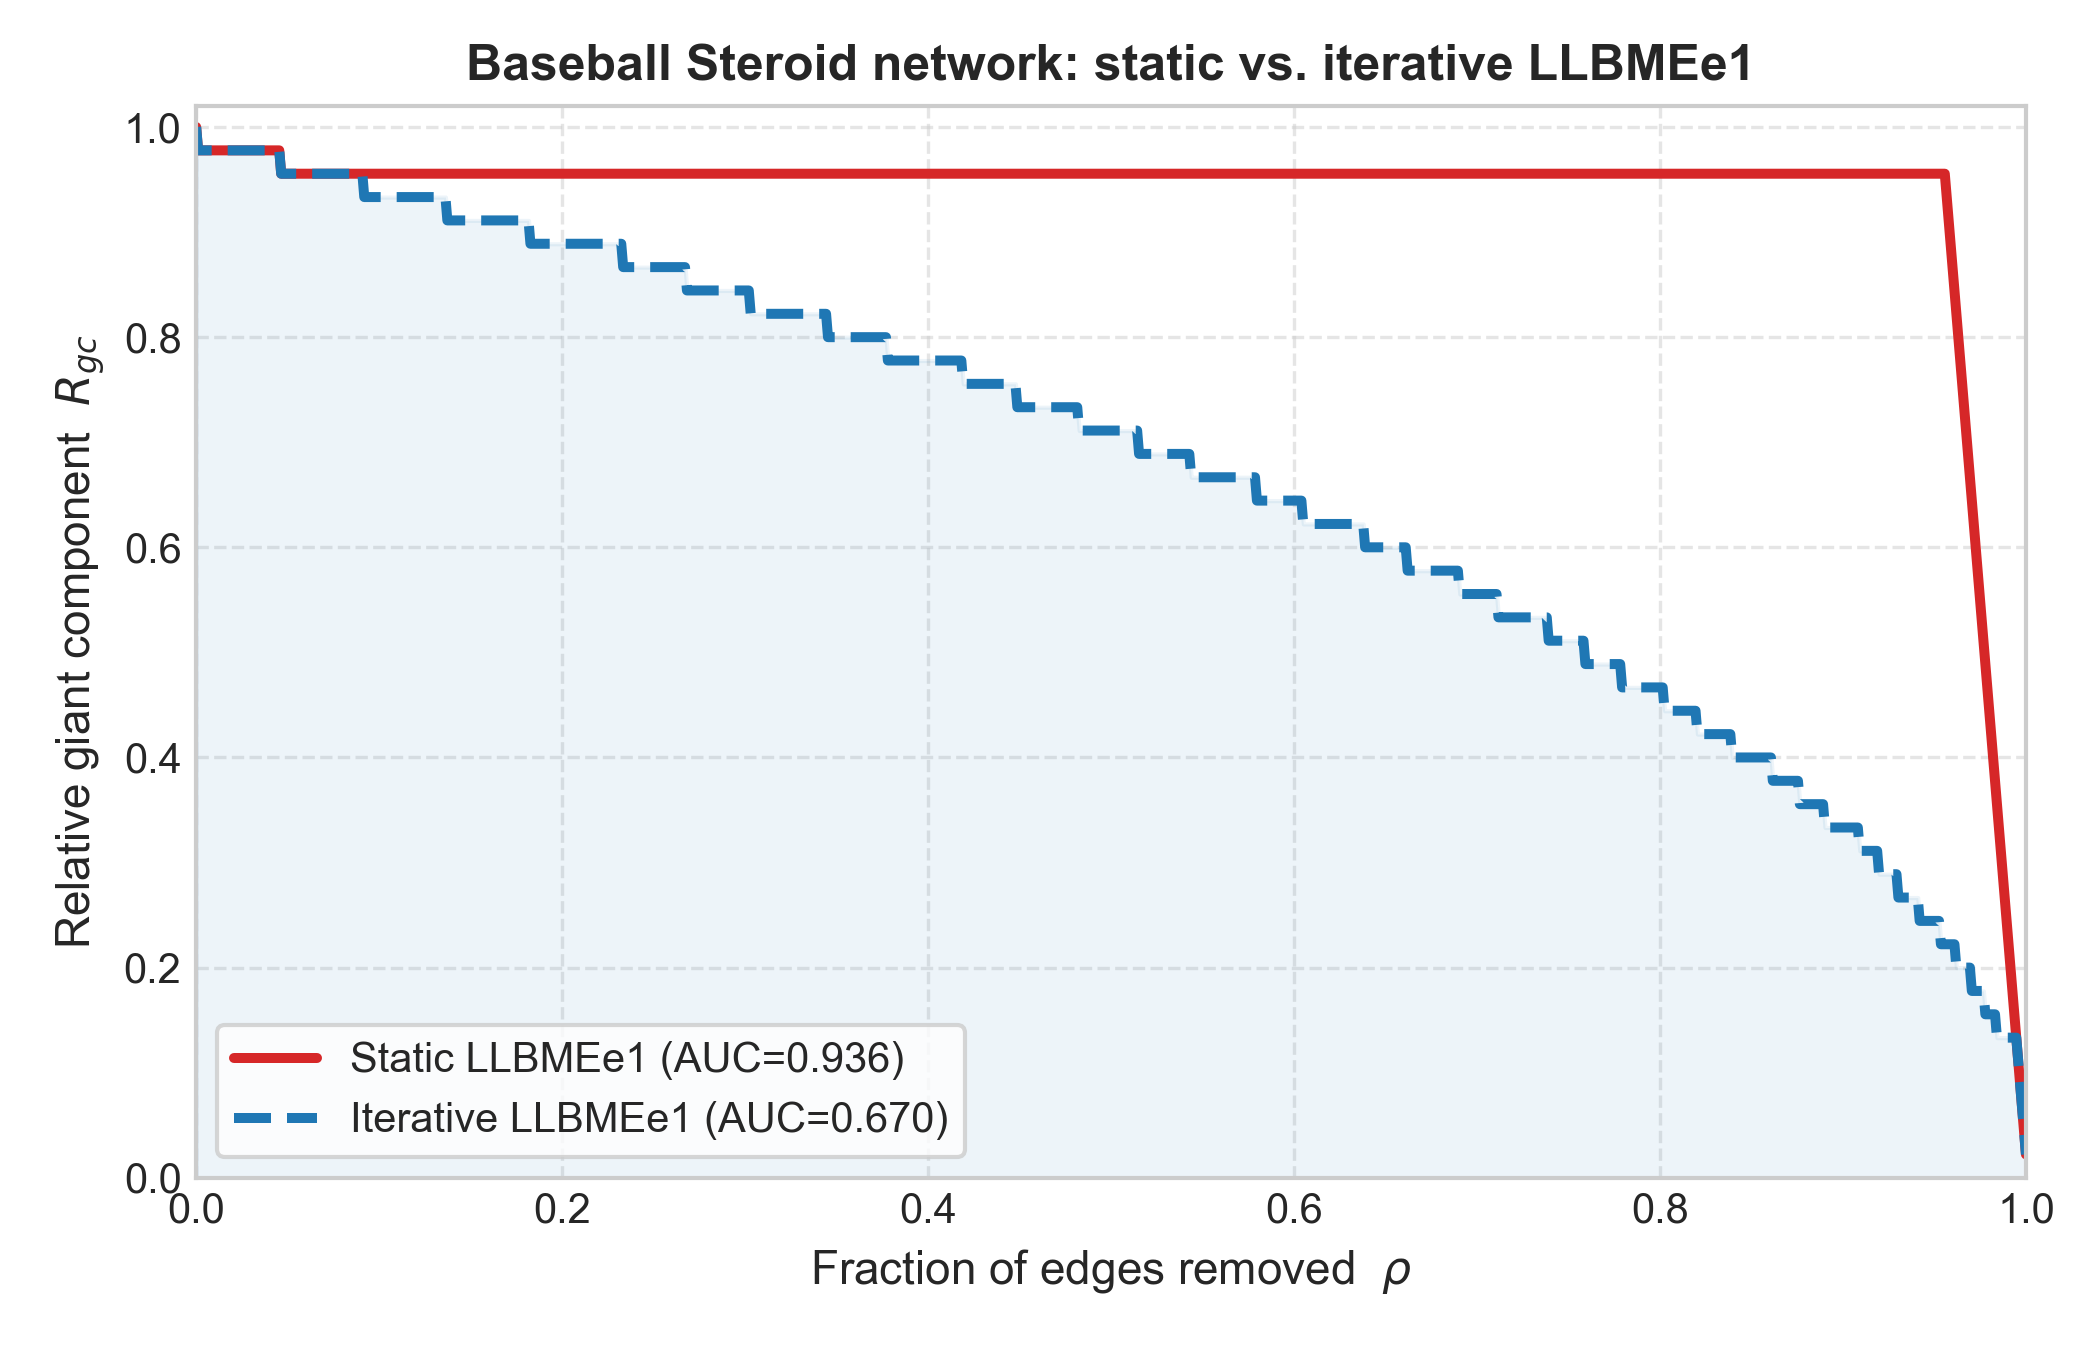
\includegraphics[width=\linewidth]{baseball_LLBMEe1.png}
\caption{LLBMEe1}
\end{subfigure}
\caption{Static (solid) vs.\ iterative (dashed) dismantling curves for the
\textbf{Baseball} network. On this near-complete graph the static metrics are
nearly tied; iteration sharply separates the betweenness-based metrics.}
\label{fig:baseball}
\end{figure}

\subsection{Urban Transport Network}
\label{sec:net-transport}
The Transport network is a large, very sparse, almost tree-like spatial graph
of $369$ nodes and $430$ edges ($\langle k\rangle=2.3$, $C=0.029$), where
connectivity is governed by a small number of bridge edges.
\Cref{fig:transport} shows its decomposition. The absolute AUC values are
the lowest of any network (the graph fragments abruptly once its bridges are
cut), and iteration helps all three metrics, most of all LLBMEe1 and LDC:
tracking the changing topology lets the iterative ranking target each cut-edge
as it becomes critical, whereas the static ranking commits to an ordering
computed before any of the tree-like structure has been exposed.

\begin{figure}[t]
\centering
\begin{subfigure}[t]{0.32\textwidth}
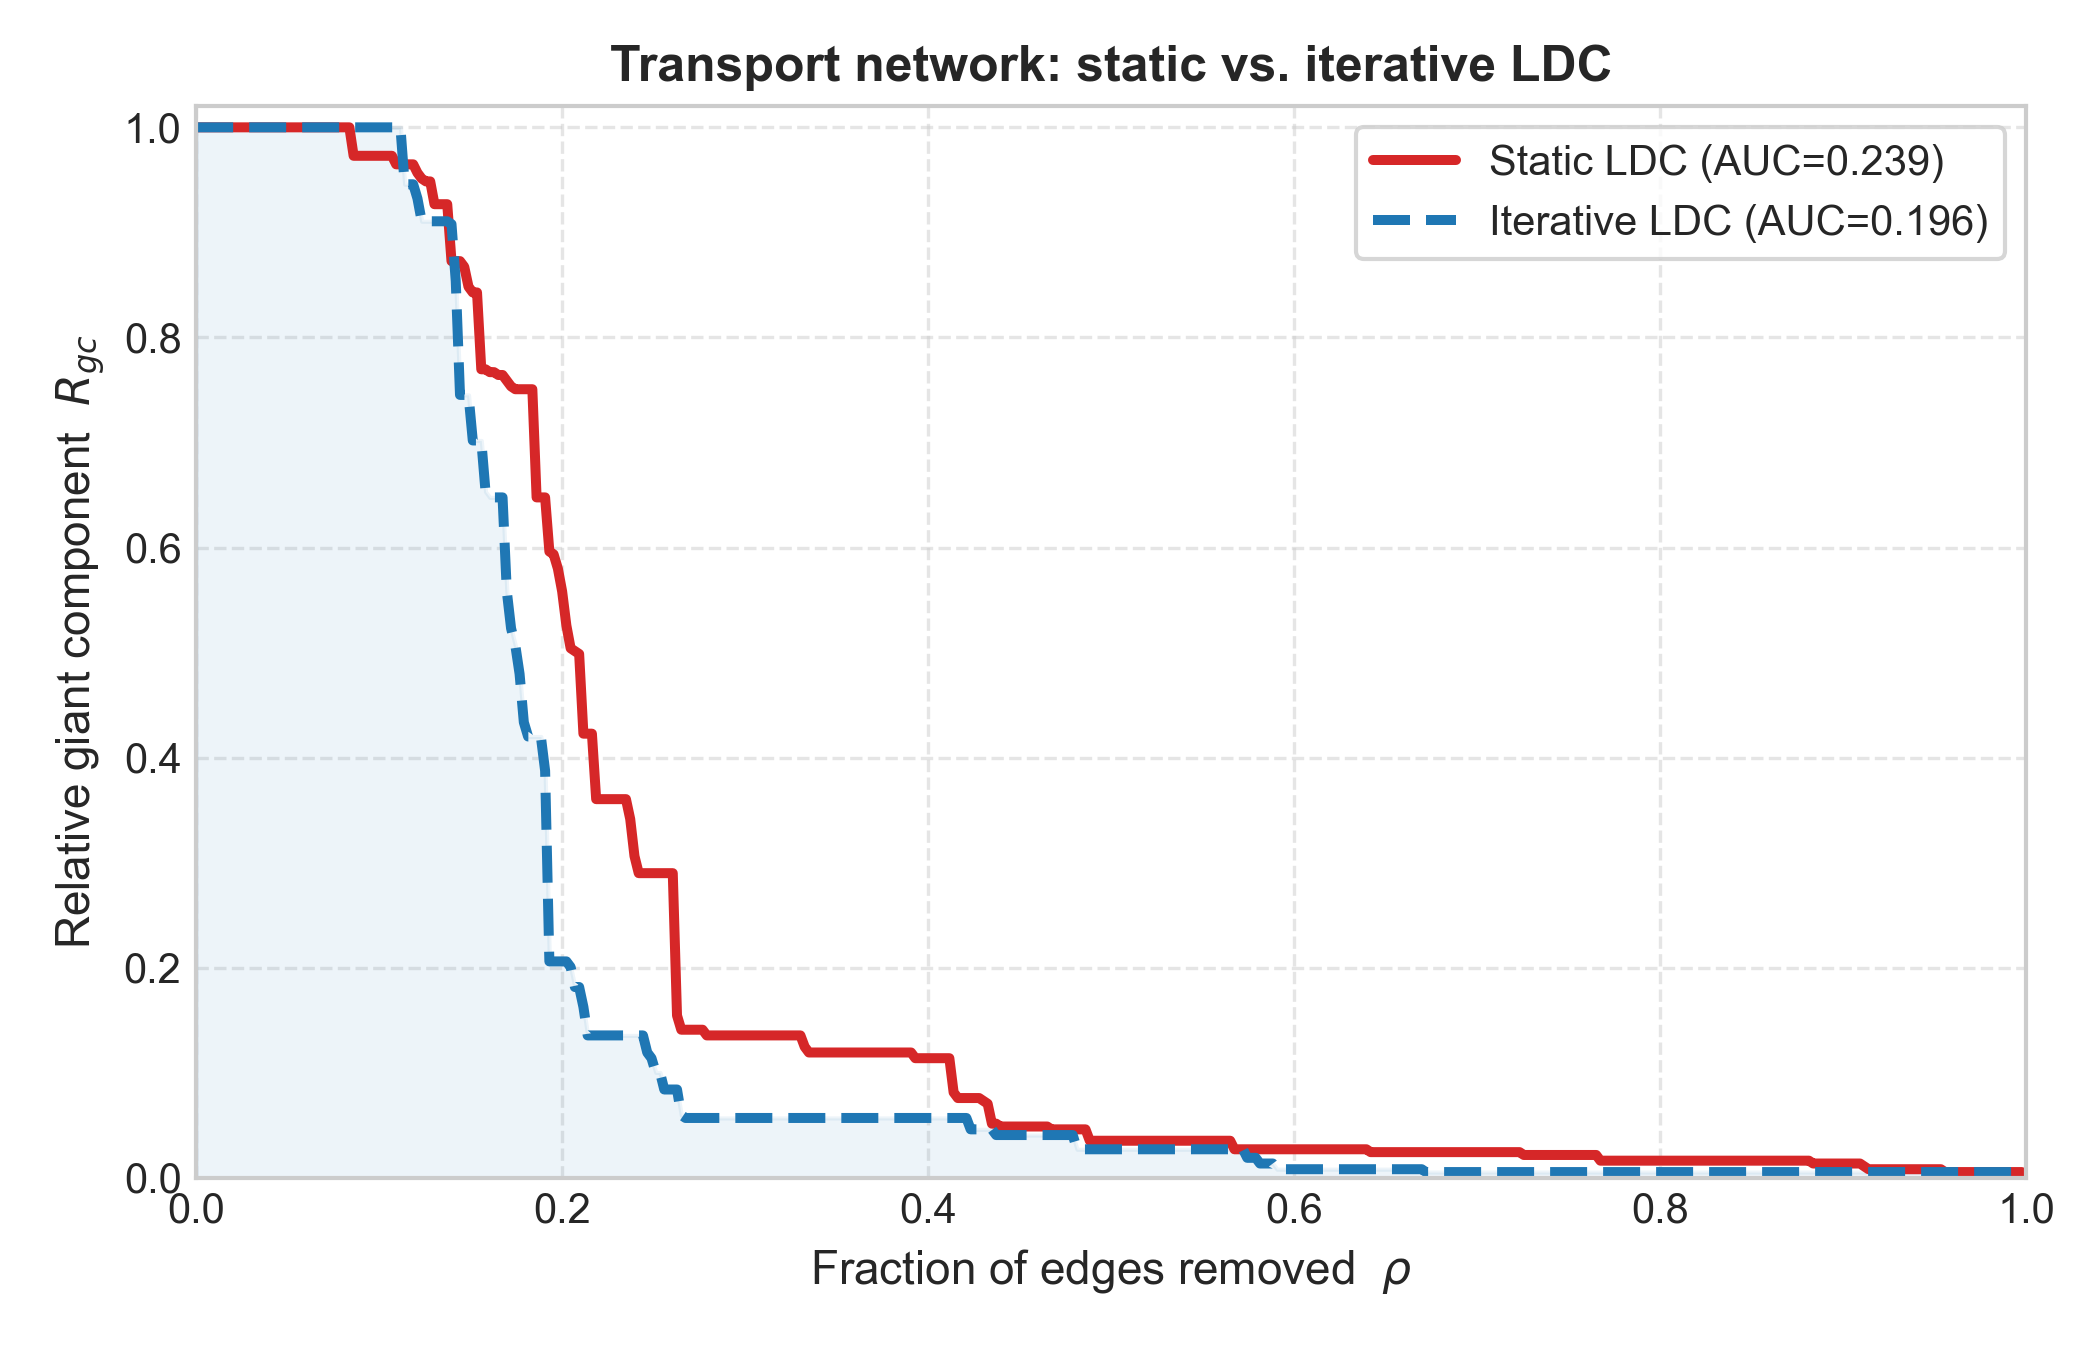
\includegraphics[width=\linewidth]{transport_LDC.png}
\caption{LDC}
\end{subfigure}
\hfill
\begin{subfigure}[t]{0.32\textwidth}
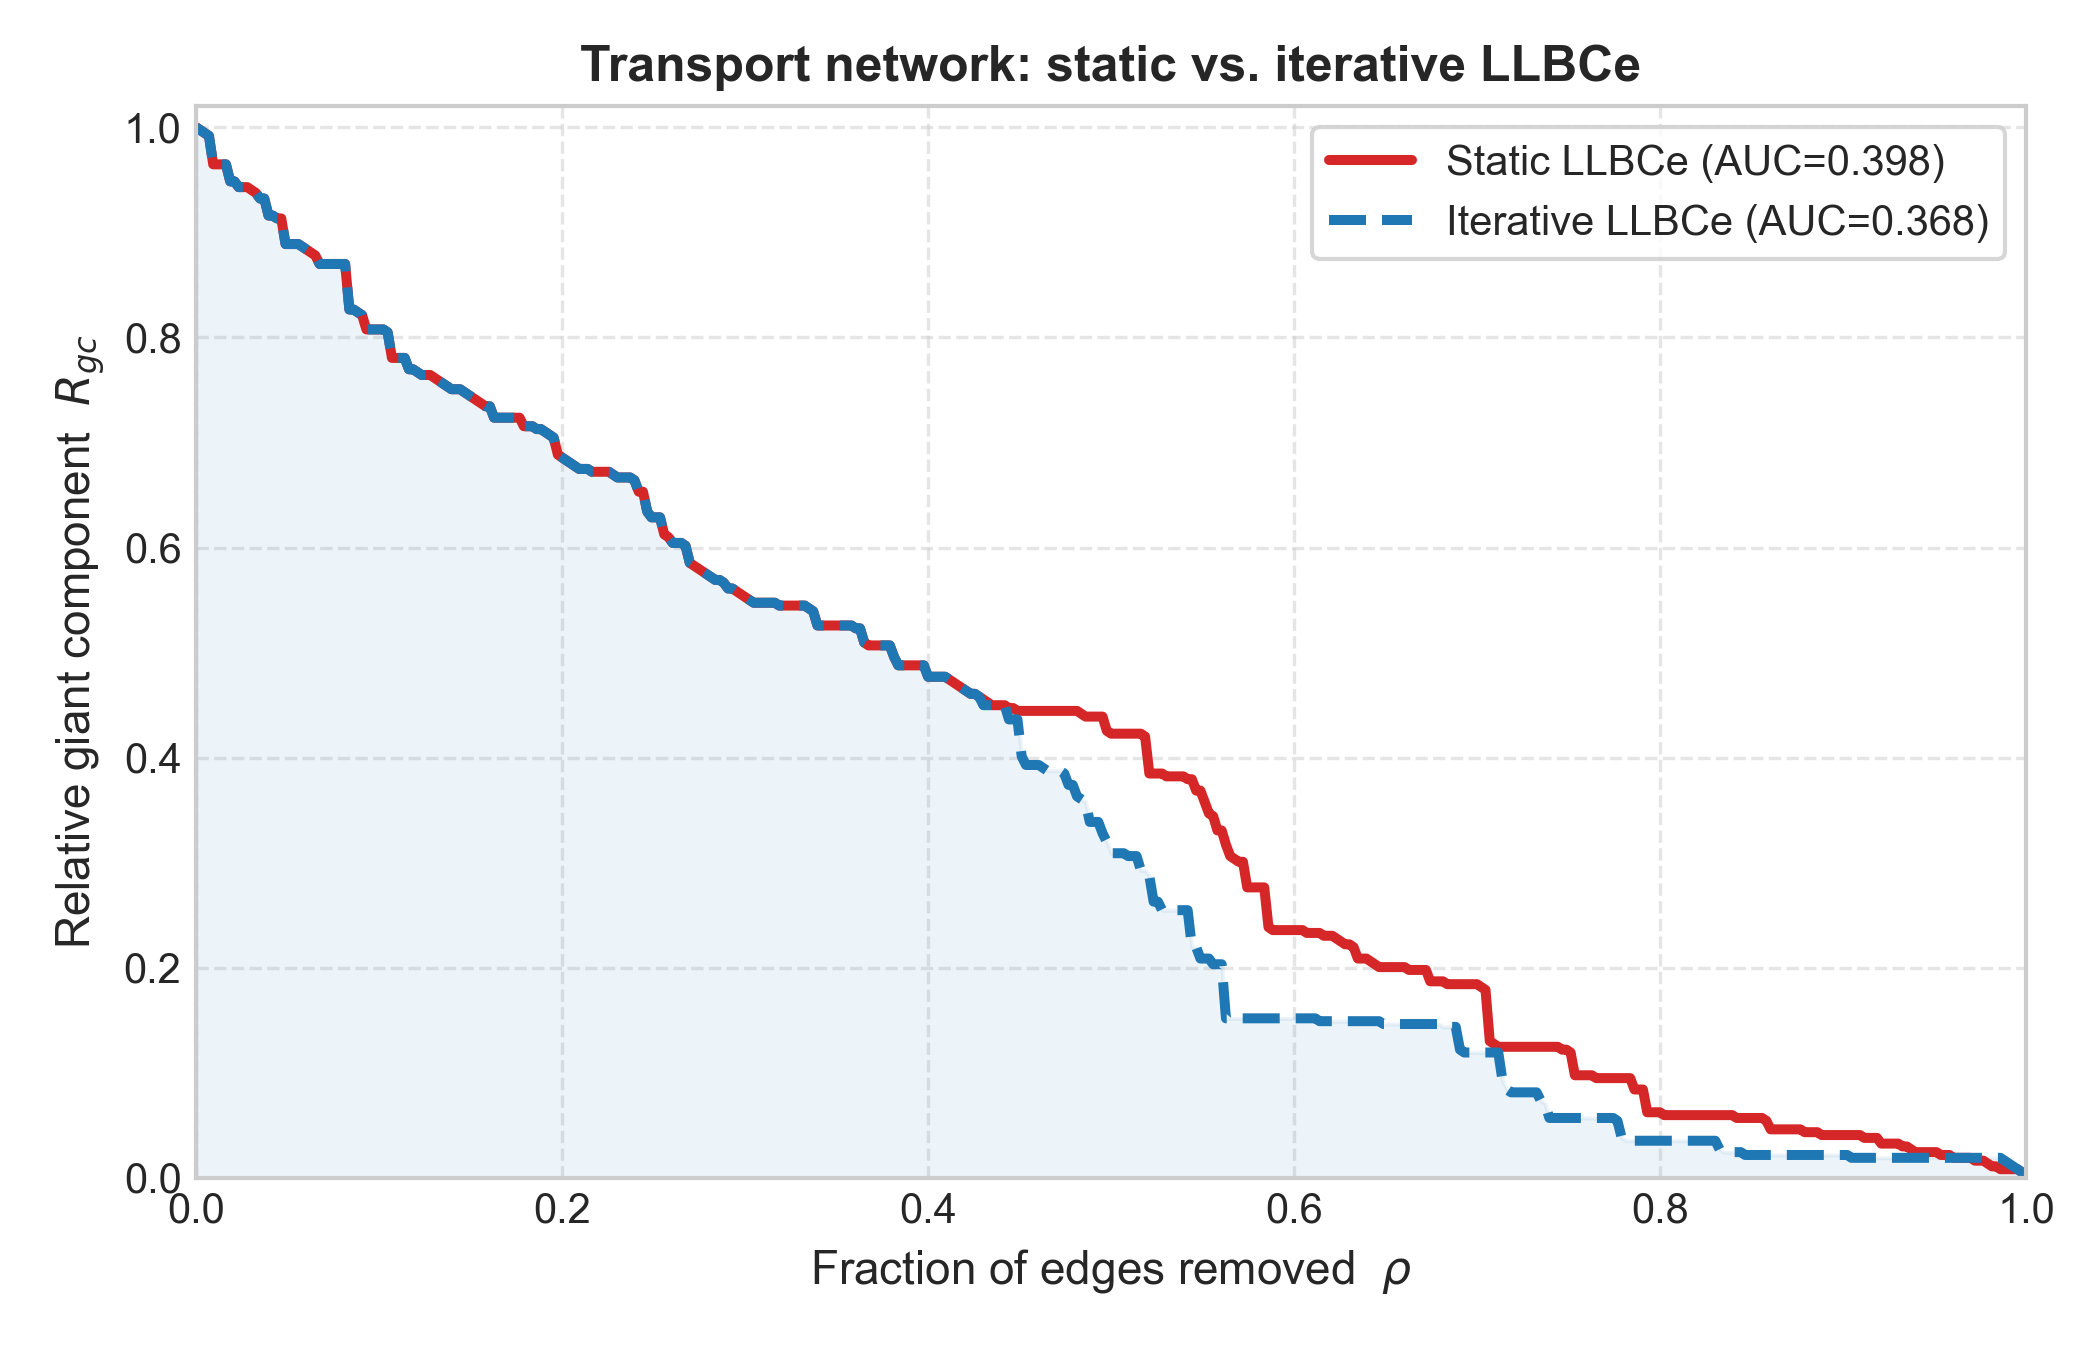
\includegraphics[width=\linewidth]{transport_LLBCe.png}
\caption{LLBCe}
\end{subfigure}
\hfill
\begin{subfigure}[t]{0.32\textwidth}
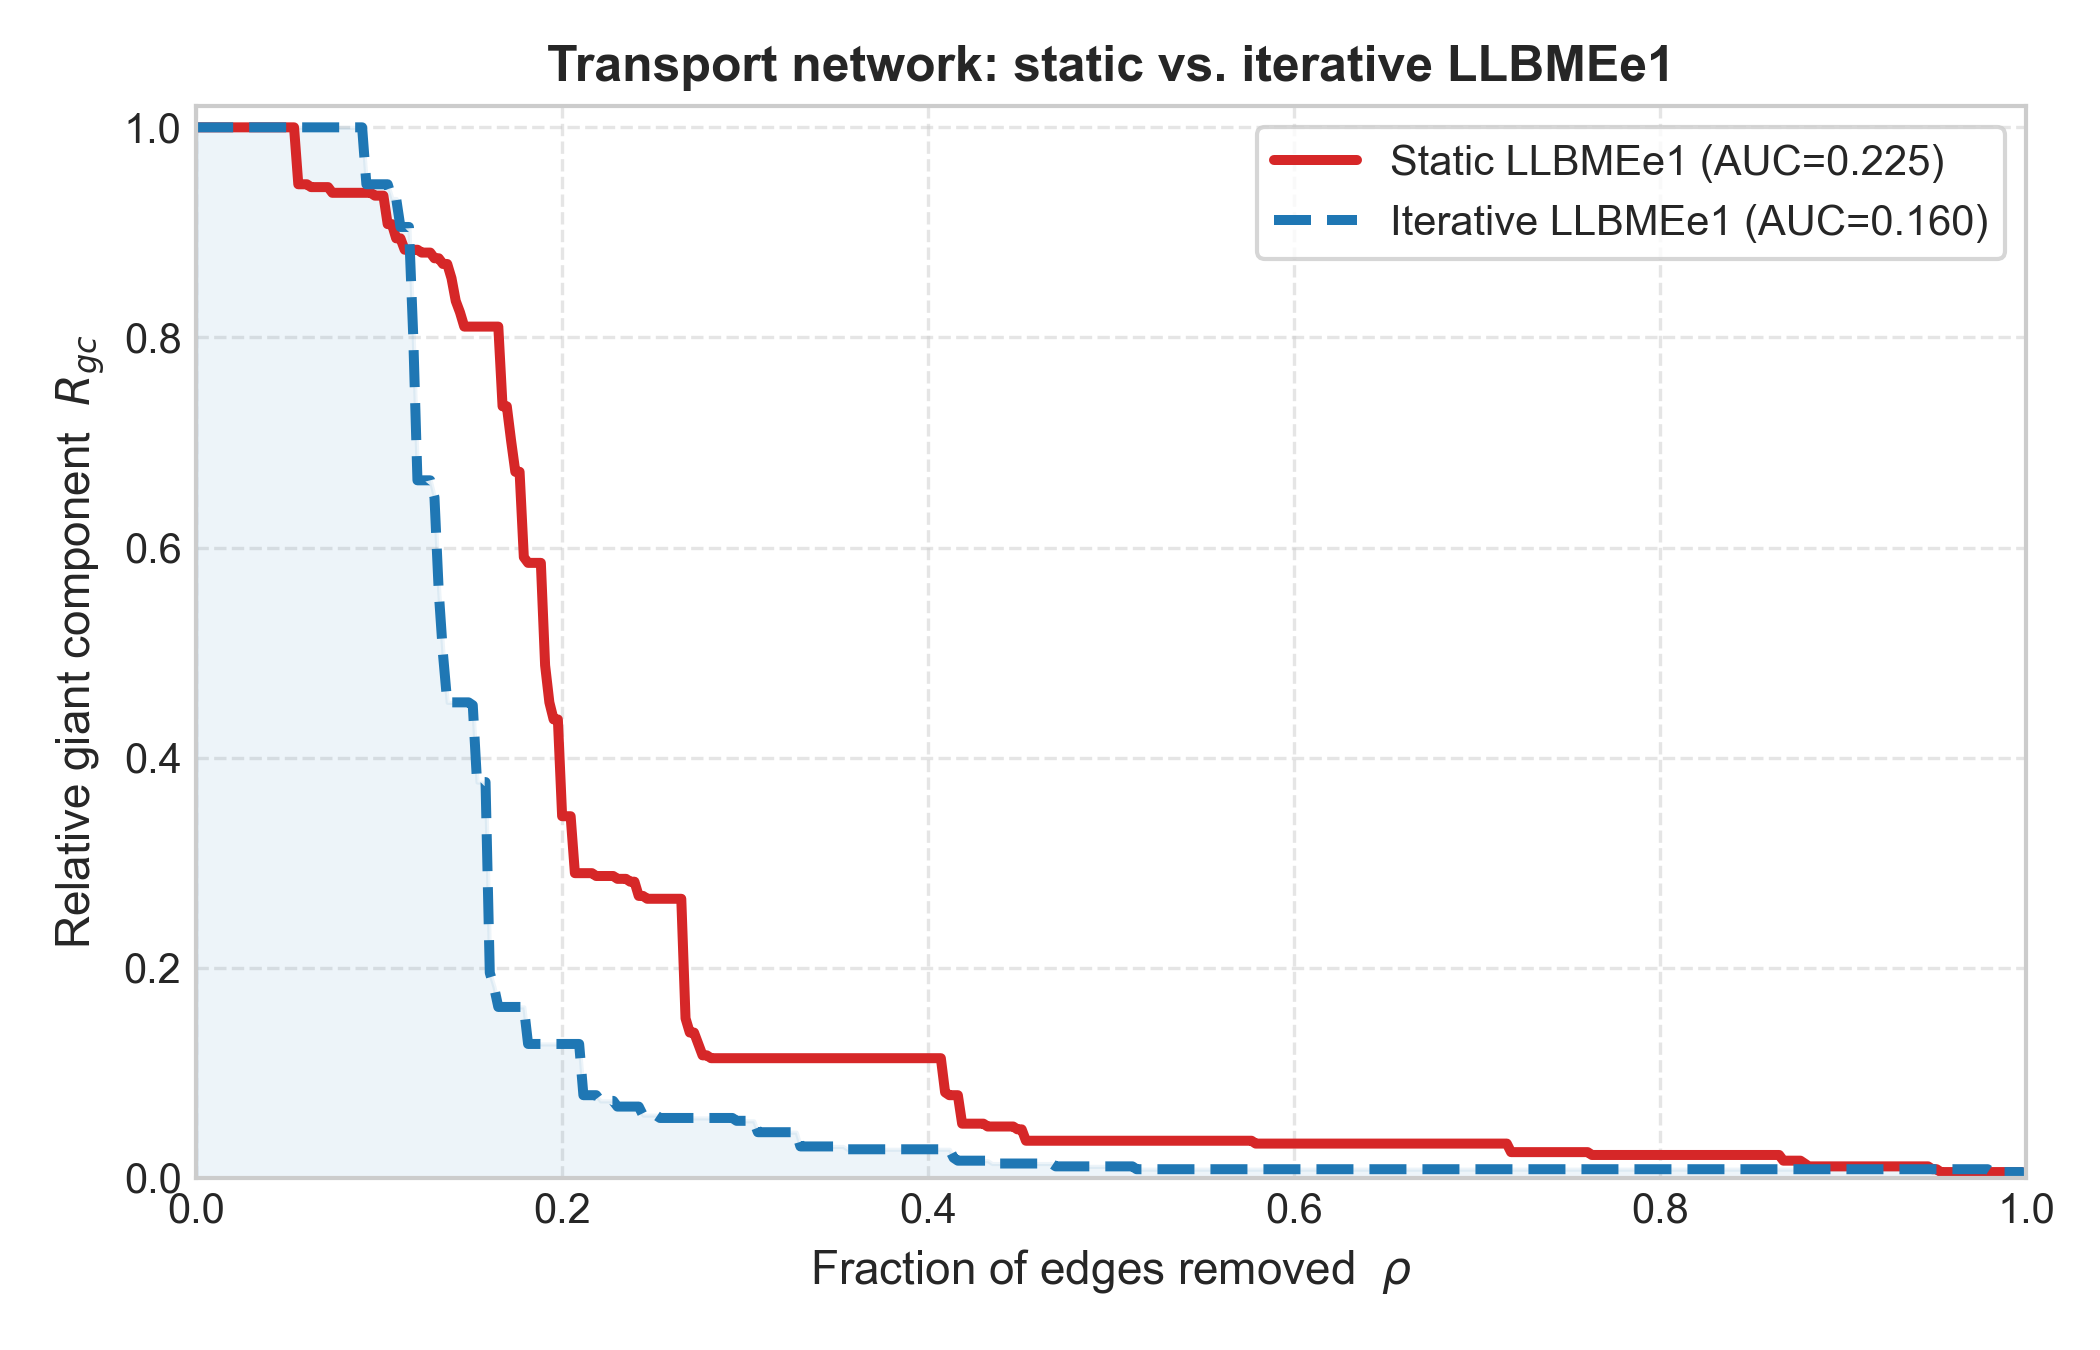
\includegraphics[width=\linewidth]{transport_LLBMEe1.png}
\caption{LLBMEe1}
\end{subfigure}
\caption{Static (solid) vs.\ iterative (dashed) dismantling curves for the
\textbf{Transport} network. Iteration helps every metric on this near-tree
graph, where connectivity hinges on a few bridge edges.}
\label{fig:transport}
\end{figure}

\section{Discussion}
\label{sec:discussion}
\Cref{tab:main} consolidates the static and iterative dismantling AUC for all
three metrics on all four networks, together with the relative change $\Delta$
(positive = the iterative variant is more efficient). Three patterns emerge.

\begin{table}[t]
\centering
\caption{Dismantling AUC (lower is better) for static and iterative LDC, LLBCe
and LLBMEe1 across the four networks. $\Delta$ is the relative AUC reduction of
the iterative variant; bold marks the two cases where iteration is slightly
counter-productive.}
\label{tab:main}
\begin{tabular}{llccc}
\toprule
Network & Metric & Static AUC & Iterative AUC & $\Delta$ (\%) \\
\midrule
\multirow{3}{*}{Jazz} & LDC & 0.9139 & 0.9356 & \textbf{$-$2.37} \\
 & LLBCe & 0.5850 & 0.4190 & $+$28.38 \\
 & LLBMEe1 & 0.7701 & 0.4339 & $+$43.66 \\
\midrule
\multirow{3}{*}{Dolphins} & LDC & 0.6750 & 0.6571 & $+$2.66 \\
 & LLBCe & 0.4548 & 0.3236 & $+$28.84 \\
 & LLBMEe1 & 0.6097 & 0.4298 & $+$29.52 \\
\midrule
\multirow{3}{*}{Baseball} & LDC & 0.9359 & 0.9600 & \textbf{$-$2.58} \\
 & LLBCe & 0.9359 & 0.6684 & $+$28.58 \\
 & LLBMEe1 & 0.9359 & 0.6704 & $+$28.37 \\
\midrule
\multirow{3}{*}{Transport} & LDC & 0.2390 & 0.1957 & $+$18.11 \\
 & LLBCe & 0.3981 & 0.3682 & $+$7.51 \\
 & LLBMEe1 & 0.2251 & 0.1595 & $+$29.10 \\
\bottomrule
\end{tabular}
\end{table}

\paragraph{LLBMEe1 benefits most from iteration.}
The mapping-entropy metric improves on every network, by an average of
\SI{32.7}{\percent} and by as much as \SI{43.7}{\percent} on Jazz. Because
LLBMEe1 couples an edge's local betweenness with the entropy of its neighbours'
betweenness, both factors shift sharply as the graph is dismantled, so a
one-shot ranking quickly becomes stale and recomputation pays off most
strongly.

\paragraph{LLBCe benefits consistently.}
Iterative LLBCe lowers the AUC on all four networks (mean \SI{23.3}{\percent}).
The largest gains are on the dense social graphs (Jazz, Dolphins, and especially
the near-complete Baseball graph, where iteration breaks the static ties), with
a smaller but still positive gain on the sparse Transport network.

\paragraph{LDC benefits only on sparse graphs.}
The degree-product metric is the exception: iteration helps clearly on Transport
($+\SI{18.1}{\percent}$) and modestly on Dolphins ($+\SI{2.7}{\percent}$), but
slightly \emph{degrades} on the dense Jazz ($-\SI{2.4}{\percent}$) and Baseball
($-\SI{2.6}{\percent}$) graphs. On graphs that dense the degree-product ordering
is already near-optimal and recomputation mostly reshuffles edges of near-equal
structural value. We report this as an honest negative result rather than
suppress it: iterative re-estimation is not universally beneficial, and its
value depends on the interaction between the metric and the topology.

\paragraph{Topology governs the benefit of iteration.}
Across all three metrics the gain from iteration tends to grow as networks become
sparser and more bridge-dominated (\cref{tab:stats}). High clustering and
density (Jazz $C=0.618$, Baseball $C=0.977$) provide local redundancy that
blunts the effect of any single removal, so the static ranking remains
serviceable; the near-tree Transport network ($C=0.029$) instead fragments
abruptly and rewards a ranking that continually tracks the changing topology.
The one consistent exception to the ``denser helps less'' rule is the
betweenness pair on Baseball, where the extreme density produces near-identical
static scores that iteration is uniquely able to disambiguate.

\paragraph{Limitations.}
The principal limitation of iterative re-estimation is computational cost.
Whereas a static ranking evaluates the metric once, the iterative variant
recomputes it after every removal, multiplying the work by the number of edges;
for the betweenness-based metrics, each recomputation itself involves repeated
local shortest-path counting. Consequently the iterative variants scale far less
favourably with network size than their static counterparts, and for
time-sensitive decomposition tasks they may not be the optimal choice. A second
limitation is the inverted-criticality sign convention of LLBMEe1
(\cref{sec:llbme}), whose log-sum can in principle change sign on edges whose
neighbours all carry raw subset-betweenness above unity; we monitor this but did
not observe it to alter ranking order materially on the four networks studied.

\section{Conclusion}
\label{sec:conclusion}
Edge criticality is a core problem in network science, and many methods address
it across networks of different sizes and types. We took the iterative
re-estimation principle, already shown to work for Deep Link Entropy and Improved
Link Entropy, and applied it to three local edge-criticality metrics: Link Degree
Centrality, Link-Local Betweenness Centrality, and Link-Local Betweenness Mapping
Entropy. Using the relative-giant-component curve and its AUC as the
decomposition-efficiency criterion, we benchmarked the static and iterative
variant of each metric on four real networks, from dense social graphs to sparse,
near-tree infrastructure.

The experiments showed that iterative re-estimation helps the two
betweenness-based metrics, LLBCe and LLBMEe1, on every network tested, by mean
AUC reductions of \SI{23.3}{\percent} and \SI{32.7}{\percent} respectively and by
up to \SI{43.7}{\percent}. It also helps the degree-product metric LDC, but only
on sparse, bridge-dominated graphs. The size of the benefit tracks network
sparsity, growing as clustering and density fall. We do not aim to undermine the
static methods, but to show that the iterative principle can add substantial
benefit for certain local metrics in certain network contexts, while reporting
honestly the two cases (LDC on the dense Jazz and Baseball graphs) where it does
not.

Future work includes combining iterative re-estimation with metric-specific
tie-breaking to recover the benefit on dense graphs and reducing the cost of
repeated local-betweenness recomputation. Extending the comparison to larger
infrastructure networks is a natural next step. These results point to when
adaptive, topology-tracking rankings outperform their static counterparts, and
they suggest further work on iterative refinements to classical edge-criticality
metrics.

\subsubsection*{Acknowledgments.}
This study was partially funded by the Personal Research Fund of Tokyo
International University, and used the NetworkEntropy research codebase.

\subsubsection*{Disclosure of Interests.}
The authors have no competing interests to declare that are relevant to the
content of this article.

\begin{thebibliography}{20}

\bibitem{newman2003structure}
Newman, M.E.J.: The Structure and Function of Complex Networks. SIAM Review
\textbf{45}(2), 167--256 (2003)

\bibitem{albert2002statistical}
Albert, R., Barab\'asi, A.-L.: Statistical Mechanics of Complex Networks. Rev.
Mod. Phys. \textbf{74}(1), 47--97 (2002)

\bibitem{xia2008attack}
Xia, Y., Hill, D.J.: Attack Vulnerability of Complex Communication Networks.
IEEE Trans. Circuits Syst. II \textbf{55}(1), 65--69 (2008)

\bibitem{braunstein2016network}
Braunstein, A., Dall'Asta, L., Semerjian, G., Zdeborov\'a, L.: Network
Dismantling. Proc. Natl. Acad. Sci. USA \textbf{113}(44), 12368--12373 (2016)

\bibitem{cheng2010bridgeness}
Cheng, X.Q., Ren, F.X., Shen, H.W., Zhang, Z.K., Zhou, T.: Bridgeness: A Local
Index on Edge Significance in Maintaining Global Connectivity. J. Stat. Mech.
\textbf{2010}(10), P10011 (2010)

\bibitem{onnela2007structure}
Onnela, J.-P., et al.: Structure and Tie Strengths in Mobile Communication
Networks. Proc. Natl. Acad. Sci. USA \textbf{104}(18), 7332--7336 (2007)

\bibitem{wang2008universal}
Wang, W.X., Chen, G.R.: Universal Robustness Characteristic of Weighted
Networks Against Cascading Failure. Phys. Rev. E \textbf{77}(2), 026101 (2008)

\bibitem{wang2017identification}
Wang, Z., He, J., Nechifor, A., Zhang, D., Crossley, P.: Identification of
Critical Transmission Lines in Complex Power Networks. Energies \textbf{10}(9),
1294 (2017)

\bibitem{ghosh2011railway}
Ghosh, S., Banerjee, A., Sharma, N., Agarwal, S., Ganguly, N.: Statistical
Analysis of the Indian Railway Network: A Complex Network Approach. Acta Phys.
Pol. B Proc. Suppl. \textbf{12}(2), 123 (2011)

\bibitem{ozaydin2021deep}
Ozaydin, S.Y., Ozaydin, F.: Deep Link Entropy for Quantifying Edge Significance
in Social Networks. Appl. Sci. \textbf{11}(23), 11182 (2021)

\bibitem{lubashevskiy2023improved}
Lubashevskiy, V., Ozaydin, S.Y., Ozaydin, F.: Improved Link Entropy with
Dynamic Community Number Detection for Quantifying Significance of Edges in
Complex Social Networks. Entropy \textbf{25}(2), 365 (2023)

\bibitem{lubashevskiy2023evolutionary}
Lubashevskiy, V., Lubashevsky, I.: Evolutionary Approach for Detecting
Significant Edges in Social and Communication Networks. IEEE Access \textbf{11},
58046--58054 (2023)

\bibitem{entropy2024llbme}
Link-Local Betweenness and Mapping-Entropy Indices for Edge Significance in
Complex Networks. Entropy \textbf{26}(4), 315 (2024)

\bibitem{gleiser2003jazz}
Gleiser, P.M., Danon, L.: Community Structure in Jazz. Adv. Complex Syst.
\textbf{6}(4), 565--573 (2003)

\bibitem{lusseau2003dolphins}
Lusseau, D., et al.: The Bottlenose Dolphin Community of Doubtful Sound Features
a Large Proportion of Long-Lasting Associations. Behav. Ecol. Sociobiol.
\textbf{54}, 396--405 (2003)

\bibitem{morselli2009crime}
Morselli, C.: Inside Criminal Networks. Springer, New York (2009)

\end{thebibliography}

\end{document}
